% ============================================================================
% thesis_bastidas.tex
% Selection and Transmission in Space: A Multiscale Price-Equation
% Decomposition of Ecuador's Formal Economy, 2017-2023.
% Compile from this folder:  tectonic -X compile thesis_bastidas.tex
% Figures are shared with the Spanish thesis (../es) and live in ../figures/.
% Each is a copy of a file under results/; thesis/sync_figures.py records
% which, and the comment after each caption repeats it.
% ============================================================================
\documentclass[conference]{IEEEtran}
% tectonic runs XeTeX, whose native TU encoding has no Times (ptm) shapes;
% forcing T1 restores real Times with working italics and bold.
\usepackage[T1]{fontenc}
\IEEEoverridecommandlockouts
\usepackage{cite}
\usepackage{amsmath,amssymb,amsfonts}
\usepackage{graphicx}
\usepackage{booktabs}
\usepackage{textcomp}
\usepackage{xcolor}
\usepackage{url}

\graphicspath{{../figures/}}

\newcommand{\Cov}{\operatorname{cov}}
\newcommand{\E}{\operatorname{E}}

\begin{document}

\title{Selection and Transmission in Space:\\
A Multiscale Price-Equation Decomposition of\\
Ecuador's Formal Economy, 2017--2023
}

\author{\IEEEauthorblockN{Victor Bastidas}
\IEEEauthorblockA{\textit{Universidad San Francisco de Quito}\\
Quito, Ecuador\\
vbastidas@estud.usfq.edu.ec}
\and
\IEEEauthorblockN{Pablo Astudillo Est\'evez}
\IEEEauthorblockA{\textit{Tutor de Tesis}\\
\textit{Universidad San Francisco de Quito}\\
Quito, Ecuador\\
pastudillo@usfq.edu.ec}
}

\maketitle

\begin{abstract}
Growth is a multi-scale phenomenon, produced by firms and places changing
at many levels of spatial organization at once. Standard macroeconomic
aggregates average over these processes: they report whether an economy
grew and by how much, but not whether growth came from units improving
themselves or from reallocation between them---two possibilities with
opposite implications for spatial inequality, a pressing question in
Ecuador, where 2 of the 804 parishes analyzed hold more than half of all
private corporations. To address this gap, we adapt to Ecuador's firm
sector the multiscale Price-equation decomposition of Kemp, F\"ursich and
Bettencourt, which splits change exactly into selection (reallocation
across units) and transmission (change within them) across nested spatial
scales. The selection term is already familiar to economics as the
Olley--Pakes covariance; asked of places rather than firms, it measures
whether activity concentrates or disperses, and because places nest and
firms do not, it can be evaluated within and between provinces, cantons
and parishes simultaneously. The decomposed quantity is the firm-weighted
mean of log real reported sales by parish, 2017--2023, taking parishes as
units and firm-count growth as fitness. The number of firms is the stock
of private corporations active in the tax registry, counted only in the
parishes, activities and months with reported sales. Selection is
persistently negative and small beside transmission: the stock of
corporations grows faster in places with lower sales. Of that selection,
84 percent lies between provinces; the component among cantons of a
province is a third of it with the same sign, and the component among
parishes of a canton is small and of changing sign. The sign of selection
and its concentration between provinces hold in every robustness test, and 88 percent of selection reflects the size of parishes in
number of firms rather than their sales per firm. In the 2019$\to$2020
step, coinciding with the pandemic, selection inverted at all three
scales, with Quito alone supplying a sixth of the reversal. This result describes
the population of the study, corporations in activities with reported
sales: what concentrated in 2020 was activity with reported sales, not the
registry of active corporations, whose stock grew at similar rates in
parishes of every size. Natural persons and the complete registry of
active corporations are different objects of study, with other units and
other weights, and their results are not comparable with those of this
work. The design is descriptive: it attributes no
causes, evaluates no interventions and observes counts grouped by place
and activity, not individual firms. We state as a policy hypothesis that
territorial instruments should be evaluated at the scale where
reallocation operates: between provinces it already favors smaller
places, though slowly (the share of the firm stock located in Quito and
Guayaquil went from 56.5 to 52.9 percent in six years).
\end{abstract}

\begin{IEEEkeywords}
Price equation, Olley--Pakes decomposition, selection and transmission,
multiscale spatial dynamics, firm demography, economic resilience,
Gibrat's law, formalization, Ecuador, COVID-19
\end{IEEEkeywords}

% ============================================================================
\section{Introduction}
% ============================================================================

In most of the developing world the majority of economic activity is still formalizing:
roughly six out of ten workers globally are informally employed, and
in Latin America the share regularly exceeds half~\cite{ilo2018}. The slow
migration of firms out of informality---\textit{formalization}---is therefore
one of the central development processes of our time, yet it is usually
measured with a single national number: how many firms registered, how much
recorded output grew~\cite{laporta2014}. That number cannot answer the
question that decides whether formalization narrows or deepens spatial
inequality: \textit{when the formal economy grows, how much of the change
comes from places growing, and how much from activity moving between
places?}

Ecuador is a clear example for that question. Between 2017
and 2023 its formal private sector expanded markedly---the stock of
private corporations grew by a factor of 1.74 while their real reported
sales grew by a factor of 1.30---and its tax authority (Servicio de Rentas
Internas, SRI) records, monthly, for every parish and every economic
activity, the two ingredients an evolutionary accounting needs: how many
formal firms there are, and what they sold in total. The analysis is
limited to private corporations, that is, firms incorporated as legal
entities: they are the units with their own legal standing, accounts and
monthly filing, and are taken here as the firmest expression of
formalization; natural persons with economic activity, far more numerous,
are outside its scope. The economy is also extremely concentrated in
space---two of the 804 parishes analyzed, central Quito and central
Guayaquil, hold over half of all formal firms (56.5 percent in 2017)---so
the difference between ``places growing'' and ``growth moving'' is not a
technicality but the substance of the country's spatial development.

The distinction matters because averages routinely fail as descriptions.
A motivating example from the data: between 2023 and 2024 (the eleven
comparable months of both years) the province of
Loja, a one-billion-dollar formal economy, recorded aggregate real sales
growth of $+0.0$ percent, and every standard robustness check (drop the
largest canton, take the median parish) confirms that number. Underneath, 34
parishes grew and 33 declined; one canton multiplied its sales 6.7 times
with an unchanged firm stock while another lost 98 percent of its formal
sales. The aggregate is not wrong---it is the truthful answer to a question
no place in Loja experienced. What is needed is a statistic that separates,
exactly and at every spatial scale, the components an average misidentifies.

This thesis builds that statistic for Ecuador by applying the multiscale
Price-equation framework developed for urban income dynamics in
Chicago by Kemp, F\"ursich, and Bettencourt~\cite{kemp2025} to a national,
firm-demographic setting. The Price equation~\cite{price1970,frank2012}
splits the change of any weighted average into a \textit{selection} term (a
covariance between relative growth and the trait) and a \textit{transmission}
term (the trait change experienced within units), with no model, no error
term, and no assumptions; the law of total covariance then splits selection
exhaustively across a nested geography. Economics has long used the closely
related Olley--Pakes decomposition~\cite{olleypakes1996,melitz2015} to
separate within-firm productivity growth from reallocation, but rarely for
places, and almost never across several spatial scales at once.

The contributions are: (i) a complete, exactly verified three-path
decomposition (Price on log sales; Olley--Pakes on the sales level; and
Olley--Pakes on the firm count itself, which doubles as a multiscale test
of Gibrat's law \cite{gibrat1931,sutton1997}) of the sales of Ecuador's
formal private sector at monthly, quarterly, and annual grain over
2017--2023, with the accounting identity holding to machine precision at
every scale; (ii) a characterization of the territorial
pattern---persistent spatial dispersion of the stock of corporations, concentrated
mostly at the between-province scale (84 percent of selection), with a
smaller component of the same sign between cantons and a small one of
changing sign between parishes, and 88 percent of it reflecting the size
of places in number of firms rather than their sales per firm; (iii) a
descriptive anatomy of the inversion of that pattern in the 2019$\to$2020
step, coinciding with the pandemic, including which city carried it and
through which economic sectors, whose scope is the population with reported activity, not the complete
registry of active corporations; (iv) a three-number ``masked growth''
detector that audits any aggregate growth figure against its own spatial
composition; and (v) a description of the relation between economic
diversification and the depth of the 2020 fall, in which sectoral breadth
is associated with the absence of extreme falls and not with a smaller
average fall. The design is descriptive: the decomposition is an
accounting identity that identifies no causes, does not attribute the
changes observed in 2020 to the pandemic, and does not demonstrate the
effectiveness of any intervention.

The remainder is organized as follows. Section II reviews the data.
Section III develops the method. Sections IV--VIII present the results:
the two margins of the expansion of the formal sector, the headline decomposition and
its scale anatomy, the 2019$\to$2020 inversion, the masked-growth audit,
and the diversification analysis. Section~IX collects the robustness
evidence, Section~X the limitations, and Section~XI concludes with policy
hypotheses.

% ============================================================================
\section{Data}
% ============================================================================

\subsection{Sources and construction}

The panel combines two SRI sources. The first is an aggregated extract of
sales declarations, obtained through a special request, with one row per
(parish $\times$ fiscal month $\times$ taxpayer type $\times$ CIIU rev.~4
activity) and total reported sales. The second is the monthly statistic of
active taxpayers, which reports the number of registered taxpayers by
(month $\times$ CIIU section $\times$ type $\times$ parish). Sales come
from the first source and the \textit{number of firms} from the second:
it is the stock of private corporations whose registration (RUC) is
active each month, net of suspensions and cancellations and not the
number ever registered, restricted to the cells (parish $\times$ CIIU section $\times$
month) in which at least one corporation filed a sales declaration.
That definition follows from the question. The paper asks how the
reported sales of the place of the average firm change, so the population
is private corporations with reported activity, and the trait (reported
sales) exists only in those cells. The count is a registry stock, not a
count of filers: a cell with a declaration may hold active corporations
that did not file that month, and the grouped counts cannot tell how
many. Active corporations in cells with no declaration are left out:
3.0 to 3.8 percent of active corporations nationally, but more than half in
parishes with fewer than ten corporations (54 percent in 2019). Counting all active corporations, with or without reported activity, is
not a variant of this definition but a different object of study, the
registry of active corporations: it gives weight to corporations whose
trait is not observed, so its results are not comparable with those of
this work and do not test them. Section~IX documents them only to mark the
scope of what is claimed here. For the same reason the vocabulary is one of net stocks:
``adding firms'' means the stock of active corporations of a place rose,
without telling new corporations from reactivated or relocated ones, and
``dispersion'' describes changes in each place's share of that stock, not
observed moves.
Natural persons and the public sector are excluded from both. The
exclusion is a condition of the method, not a simplification: the
decomposition weights each place by its number of units and assumes the
units are comparable, and across taxpayer types they are not. In 2017 the
panel holds 117{,}290 private corporations selling \$1.15 million each;
built the same way, natural persons are 1.33 million taxpayers selling
\$31{,}000 each, and the public sector is 1{,}667 entities created by
administrative decision rather than market entry. Run on each group, the
2017$\to$2023 population-path selection is $-0.0270$ for private
corporations, $-0.0005$ for natural persons and $+0.0679$ for the public
sector. Pooled in one panel (1{,}013 parishes), natural persons are 91.6
percent of the units and 21.5 percent of sales, and private corporations
8.3 percent of the units and 70.0 percent of sales. Natural persons are
the majority of units in every parish (94.9 percent in the median one), so
they set both the weights and the fitness: the growth of the pooled
number of units correlates $0.99$ with theirs and $0.19$ with that of
corporations. The pooled result is therefore theirs (selection $-0.0021$,
less than a tenth of the corporations' value). Pooling would not widen the analysis, it would change its subject. The
pooled results are therefore not an alternative or provisional version of
the results of this work, nor a sensitivity test: they describe another
population (taxpayers with a registration, overwhelmingly natural
persons), with other units, other weights and another fitness, and belong
to a different study, not comparable with the data and the construction
used here.
Sales are
the extract's total (\texttt{V\_VTX}), which includes exports: the object
measured is the formal activity of the firms domiciled in a place,
whatever the destination of the sale, and removing exports would shrink
precisely the exporting provinces (31 percent of formal sales in El Oro
and 30 percent in Manab\'i in 2019, against 2 percent in Quito);
Section~IX shows the results do not depend on this choice. Of the
3{,}726{,}283 private-corporation rows of the extract, 38.3 percent have
a blank sales field---cells with taxpayers in which no corporation
declared sales that month---and are excluded, never turned into zeros;
the remaining 2{,}298{,}602 rows all carry positive sales. The raw
geography is crosswalked to the official INEC-DPA codification---the
6-digit code \texttt{PPCCPP} nests parishes in cantons in provinces---with
manually audited overrides; monetary values are deflated to constant-2025
US dollars with national CPI factors. The measure of activity is gross
reported sales, not value added.

Coverage runs from January 2017 to December 2024, except November 2024,
which the active-taxpayer statistic lacks. The main analysis covers the
seven complete years 2017--2023; comparisons that reach 2024 use the same
eleven months (January--October and December) at both ends of the window.
After cleaning, the window 2017--2023 contains 804 parishes with formal
activity in 220 cantons in 24 provinces. Parish-year firm counts are the
mean of the monthly stocks; sales are summed over the year. A window
keeps \textit{survivor} parishes only---present with a positive firm
stock and more than \$1{,}000 of real annual sales at both
endpoints---which removes indefensible near-empty cells (survivors hold
99.8 percent of the firm stock; a sensitivity sweep over the floor appears
in Section~IX). Ecuador offers three further advantages as a case study:
full dollarization (no exchange-rate deflation ambiguity), a single
national tax authority (uniform registration incentives), and a period
containing both a strong formalization drive and a large common shock.

\subsection{What the data cannot say}

The unit of observation is a place-and-activity, not a firm. Individual
firm dynamics are invisible: the data reveal the \textit{stock} of active
corporations per cell per month, so net entry is observable and gross
entry/exit flows are not, and there are no birth or death terms in the
decomposition---it speaks about the reallocation of \textit{continuing}
formal activity. A corporation stays active in the registry until it
suspends or cancels its registration, so the stock can overstate the
number of operating firms and smooth their declines. Location, activity
and type follow the taxpayer registration in force at the extraction
date: a taxpayer that moved appears at its current domicile in every
year, and a headquarters can carry activity produced elsewhere
(Section~VII turns this caveat into an instrument). The informal economy
is invisible by construction.

% ============================================================================
\section{Method}
% ============================================================================

Notation follows the source framework~\cite{kemp2025}. Fix a parent unit
$j$ (a canton, a province, or the country) with children $k$ (its parishes,
cantons, or provinces). Let $n_k$ and $n_k'$ be the child's firm stock at
the start and end of a window of $\Delta t$ years, $f_k = n_k / \sum_l n_l$
the \textit{initial firm share}, $y_k$ real total sales, and
$\E_j[x_k] = \sum_k f_k x_k$ the firm-weighted mean over the children of
$j$---the only averaging operator used. Fitness is the firm-count growth
factor $w_k = n_k'/n_k$, and \textit{relative} fitness is
$\bar w_k = w_k / w_j$ with $w_j = \E_j[w_k]$, centered on one. The trait
is $z_k = \ln y_k$ at the parish level; a higher-level unit inherits the
firm-weighted mean of its children's traits, $z_j = \E_j[z_k]$, not the log
of its total.

\subsection{The Price identity}

An average can rise for two reasons: every unit improved, or nothing
changed except \textit{who counts}. The final firm share of a child is
exactly its initial share retilted by relative fitness,
$f_k' = f_k \bar w_k$; substituting $z_k(t_1) = z_k(t_0) + \Delta z_k$
into the final average and regrouping once yields the Price
equation~\cite{price1970}:
\begin{equation}
\gamma^{p}_j \equiv \frac{\Delta \E_j[z_k]}{\Delta t}
= \underbrace{\frac{1}{\Delta t}\Cov_j\!\left(\bar w_k,\, z_k\right)}_{S^{p}_{k\to j}\ \text{(selection)}}
+ \underbrace{\E_j\!\left[\bar w_k \frac{\Delta z_k}{\Delta t}\right]}_{T^{p}_{k\to j}\ \text{(transmission)}} .
\label{eq:price}
\end{equation}
This is an identity, not a model: it holds for any population, any trait,
and any window, with no residual. Selection is nonzero only if firm growth
lines up with the hierarchy of total sales---firms forming in places with
systematically higher or lower total sales than the incumbents'
locations. Transmission is the growth places experienced internally,
weighted by where firms ended up (since $f_k \bar w_k = f_k'$, the
transmission term is the trait change under \textit{final} shares, while
selection prices where each unit started).

One sign convention governs everything that follows: \textit{a negative
selection term does not mean decline}. It means new formal firms are
appearing faster in places with lower total sales---spatial dispersion,
arguably good news---and it carries a minus sign because the average
firm's environment has lower total sales when the periphery gains weight.
The sign is a direction of reallocation.

The trait also admits an exact partition that the results use. A parish's
total sales are its number of firms times its sales per firm, so
$\ln y_k = \ln n_k + \ln (y_k/n_k)$; and because a covariance is linear in
the trait, every term of \eqref{eq:price}, and of its multiscale version,
is the sum of two: the one obtained with the parish's size in number of
firms, $\ln n_k$, as the trait, and the one obtained with its sales per
firm, $\ln (y_k/n_k)$. The size part of selection,
$\Cov_j(\bar w_k, \ln n_k)/\Delta t$, is exactly zero under Gibrat's
law~\cite{gibrat1931}; the per-firm part says whether firms form where
each firm sells more or less. The distinction matters for the reading: a
parish with low total sales may simply be a parish with few firms, not a
parish where firms sell little.

\subsection{The Olley--Pakes decomposition}

The Olley--Pakes decomposition~\cite{olleypakes1996} has the same
skeleton with the roles of growth and level exchanged: instead of tilting
the trait by relative fitness, tilt the growth rate by relative size.
With relative sales $\hat y_k = y_k / \E_j[y_k]$ and empirical sales
growth $\gamma_k = \Delta \ln y_k / \Delta t$, the \textit{income path}
is
\begin{equation}
\gamma^{y}_j = \E_j[\hat y_k\, \gamma_k]
= \underbrace{\Cov_j(\hat y_k, \gamma_k)}_{S^{y}_{k\to j}}
+ \underbrace{\E_j[\gamma_k]}_{T^{y}_{k\to j}} ,
\label{eq:op-inc}
\end{equation}
an average of sales growth rates in which each parish is weighted by its
firm share times its sales, split into a reweighting gap (do places with
more sales out-grow small ones?) and the mean growth weighted by firms
alone. The \textit{density path} replaces sales with the
firm count itself: with $\hat n_k = n_k / \E_j[n_k]$ and firm-count
growth $h_k = \Delta \ln n_k / \Delta t$,
\begin{equation}
\gamma^{n}_j = \E_j[\hat n_k\, h_k]
= \underbrace{\Cov_j(\hat n_k, h_k)}_{S^{n}_{k\to j}}
+ \underbrace{\E_j[h_k]}_{T^{n}_{k\to j}} .
\label{eq:op-den}
\end{equation}
The density path contains no revenue variable at all, and it has a sharp
null: under Gibrat's law~\cite{gibrat1931}---every place growing its firm
stock at the same rate---the covariance in \eqref{eq:op-den} is
identically zero. Its selection term is therefore a direct test of
proportional growth, signed by whether the dense ($+$) or the sparse
($-$) places win, and the multiscale split below localizes \textit{at which
scale} proportionality fails.

Three reference points summarize the paths. Population-path selection is
zero when the growth of the firm stock is unrelated to prior total sales; income-path
selection is zero when size carries no growth information (the classic
allocative term); density-path selection is zero exactly under Gibrat's
law. In all three, the weighting measure is the \textit{initial firm
share} $f_k$, and every tilt ($\bar w_k$, $\hat y_k$, $\hat n_k$) is a
ratio centered on one, so every selection term is dimensionless by
construction. The only asymmetry between the paths concerns time: the
population path's trait is a log level and carries no rate, so
\eqref{eq:price} divides by elapsed time once; the growth variables of
\eqref{eq:op-inc}--\eqref{eq:op-den} are already rates. Interpretively,
the population path decomposes the \textit{change of an average} while the
Olley--Pakes paths decompose \textit{averages of changes}.

The totals of the Olley--Pakes paths need a reading caveat. In the
original application~\cite{kemp2025} the level is income per household,
so the weight $f_k \hat y_k$ is each place's share of total income. Here
the level is the parish total (its sales or its firm count), and the
weight $f_k \hat y_k$ or $f_k \hat n_k$ counts size twice: Quito and
Guayaquil, which hold 56.5 percent of firms and 64.2 percent of sales,
receive 98.1 percent of the weight on the income path and 97.6 percent on
the density path. Their totals for 2017--2023 ($+0.0315$ and $+0.0826$ per
year) are therefore averages dominated by those two parishes, not the
aggregate growth of sales ($+0.0441$ per year) or of the firm stock
($+0.0922$). Their selection terms keep a precise but narrower reading:
they compare the growth of the two metropolitan areas with that of the
firm-weighted average parish. The population-path total, $+0.0226$ per
year, is the change in the firm-weighted mean of log parish sales.

\subsection{The multiscale split}

Ecuador nests: parishes in cantons in provinces in the country. Because a
parent's trait is the firm-weighted mean of its children's traits, each
child obeys the same identity \eqref{eq:price} as its parent; substituting
the child's identity into the parent's transmission term, once per level,
makes a new selection term fall out at each scale. Writing
$X_{l\to j} = \E_j[X_{l\to k}]$ for a term averaged up through
intermediate levels, the national population-path growth reads
\begin{equation}
\gamma^{p}_{ec} =
S^{p}_{pr\to ec} + S^{p}_{ca\to ec} + S^{p}_{pa\to ec} + T^{p}_{pa\to ec},
\label{eq:multiscale}
\end{equation}
selection \textit{between provinces}, plus selection \textit{among cantons
within their provinces}, plus selection \textit{among parishes within their
cantons}, plus every parish's own transmitted growth. This is the law of
total covariance: the algebra distributes selection exhaustively across
scales with no overlap and no assignment by assumption. In the
implementation the residual of \eqref{eq:multiscale} sits at machine
precision ($\sim 10^{-17}$) in every window; the Olley--Pakes paths
normalize by their own level means at each scale, so their scale splits
are computed analogously but the exact telescoping property is a feature
of the population path.

\subsection{Selection as a picture}

A weighted covariance is a weighted regression slope times a variance.
Plotting each parish as a point at (initial trait $z_k$, relative fitness
$\bar w_k$) with dot area equal to its firm share, the firm-weighted
regression line passes through the point $(\bar z, 1)$ by construction,
and \textit{selection equals its slope times the trait variance}. The tilt
of the cloud is not an illustration of the statistic---it \textit{is} the
statistic, and recomputing it point by point from the micro data
reproduces the pipeline's output to machine precision. Each parish's
contribution decomposes as
\begin{equation}
S_k = f_k \,(\bar w_k - 1)\,(z_k - \bar z)/\Delta t ,
\label{eq:contribution}
\end{equation}
share $\times$ did-it-gain-firm-share $\times$
does-it-have-higher-total-sales-than-average,
which is the anatomy used throughout Sections~V--VII to name who carries
each effect.

\subsection{Implementation}

The pipeline (Python, plain pandas) prepares the clean panel, computes
per-window transition tables, and runs all three paths at any time
grain---monthly, quarterly, or annual windows, consecutive or
year-over-year---through a single driver importing the Chicago engine of
\cite{kemp2025} unchanged. The density path is a second run of the engine
with the log firm count as the trait; the Price output of that same run
is the size part of the trait partition. Seasonality is handled by
construction rather than filtering: the monthly analysis uses 72 rolling
twelve-month windows, so every comparison is season-matched exactly.
Certification plots reconstruct each unit's left-hand side from its
decomposed right-hand side at every level and path; all points lie on the
identity diagonal with $R^2 = 1.0000$ and residuals at $10^{-16}$.

The decomposition is an accounting identity, not a structural model. It
separates the observed change exactly into selection and transmission and
locates each at a scale, but it identifies the causes of neither. In
particular, comparisons between the 2019$\to$2020 step and the others are
descriptive: they show that the year behaved differently, and in what,
without attributing the difference to the pandemic, because there is no
counterfactual.

% ============================================================================
\section{The Formalization Wave on Two Margins}
% ============================================================================

\begin{figure}[!t]
\centering
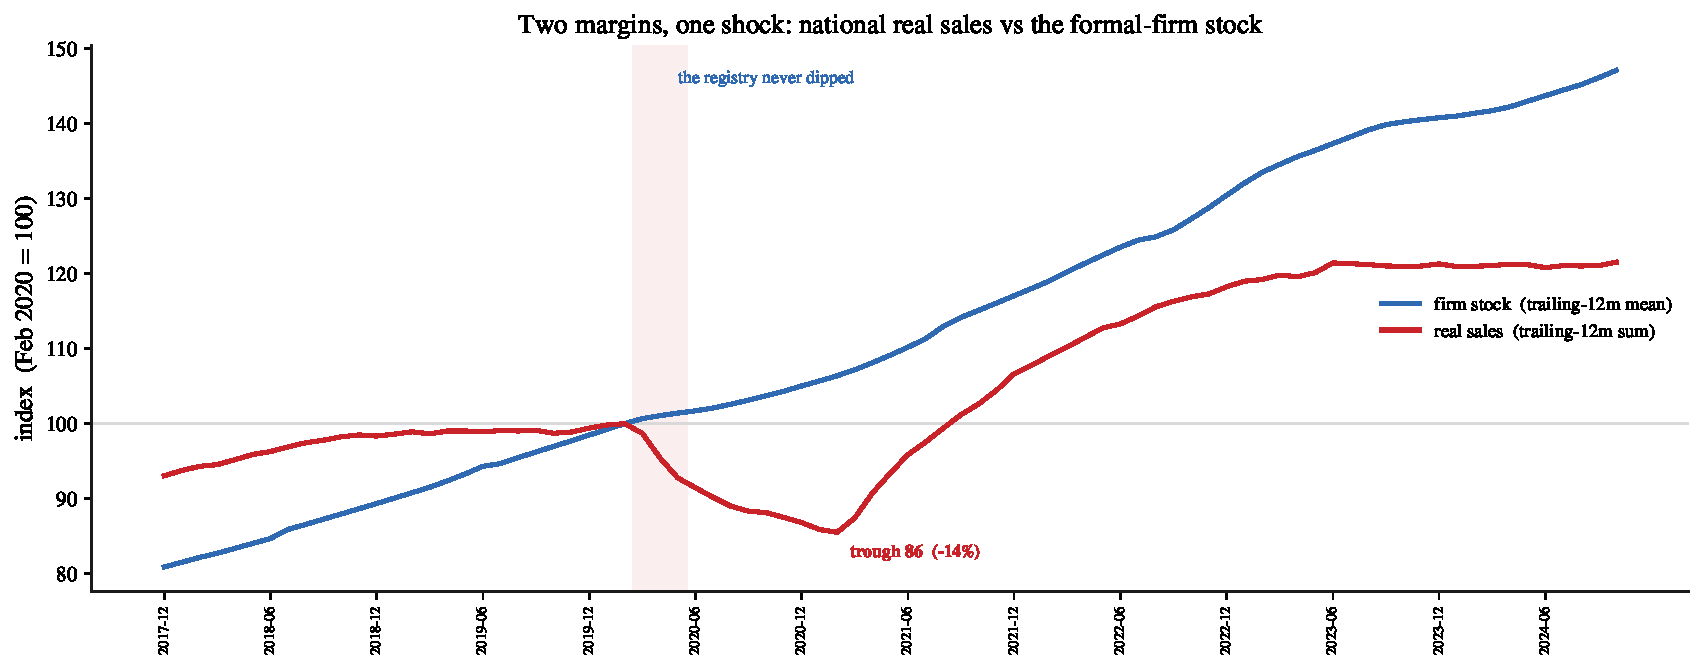
\includegraphics[width=\columnwidth]{two_margins.pdf}
\caption{The two margins through the pandemic: trailing-twelve-month
national real sales (red) fell to 86 percent of the February-2020 level,
while the formal-firm stock (blue) never dipped below its pre-shock
level.}
\label{fig:twomargins}
\end{figure}
% source: results/story/fig3_two_margins.pdf

Between 2017 and 2023 the formal firm stock grew from roughly 117,000 to
204,000 ($\times 1.74$) while real sales grew from \$134 to \$175 billion
($\times 1.30$): a horizontal expansion with a vertical cost, since real
sales per firm fell about 25 percent over the window---in every year
except the 2021 rebound. Total sales decompose exactly as
\begin{equation}
\Delta \ln(\text{sales}) = \Delta \ln(\text{firms}) +
\Delta \ln(\text{sales per firm}),
\label{eq:margins}
\end{equation}
\newpage
the extensive and intensive margins, and the two behave as different
economic objects throughout the sample. Fig.~\ref{fig:twomargins} shows
the starkest case: through a year-over-year sales trough of $-46$ percent
in April 2020, the national firm stock never fell below its pre-shock
level, and in the lockdown year itself firms grew $+6.7$ percent while
real sales fell $-12.7$ percent.

\begin{figure}[h!]
\centering
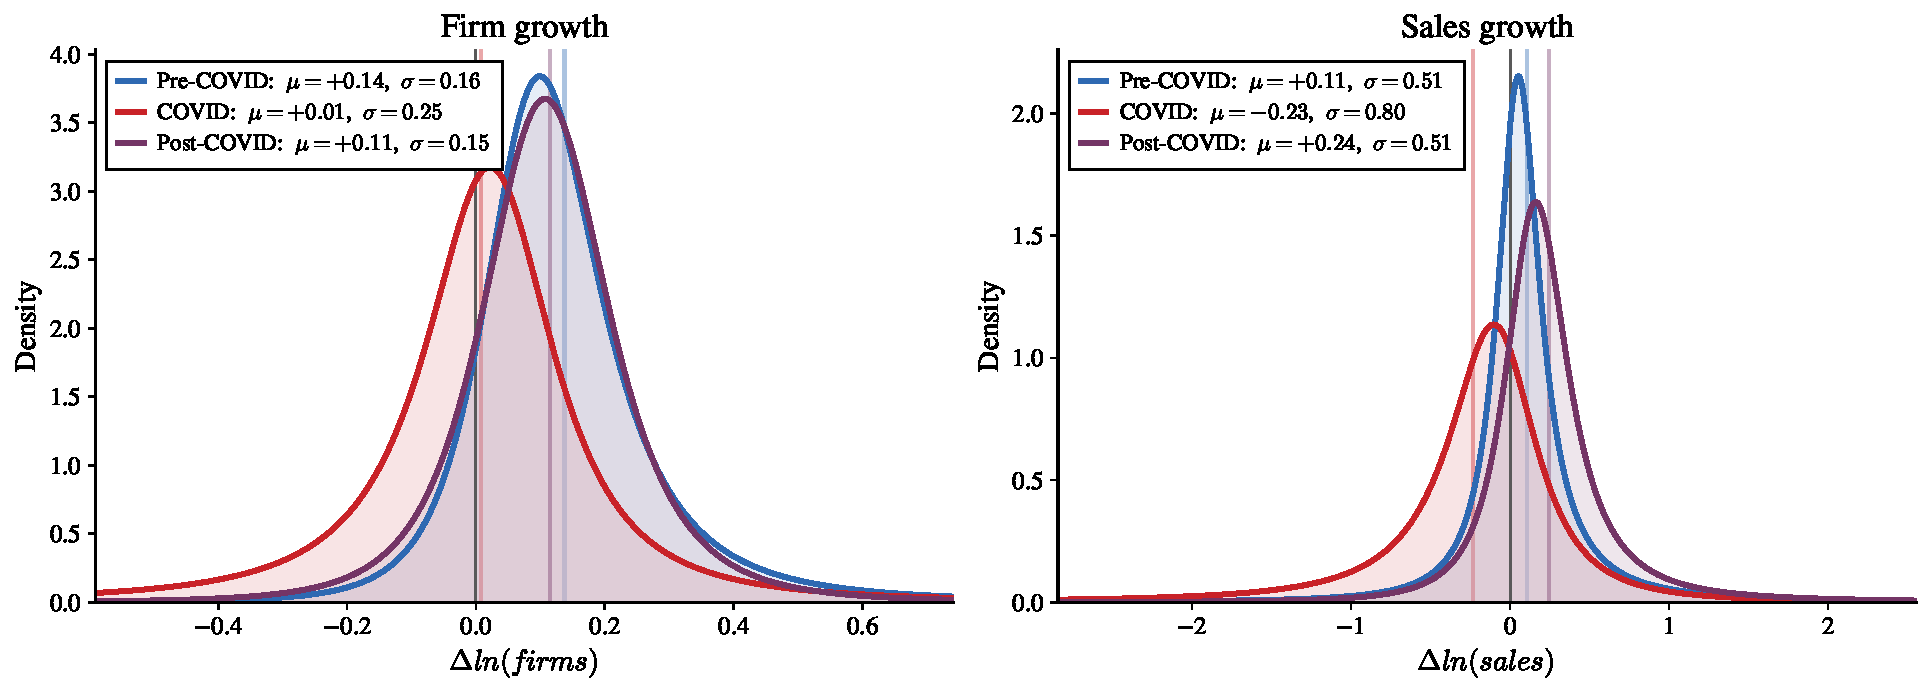
\includegraphics[width=\columnwidth]{dist_overlay_eras.pdf}
\caption{Cross-parish growth-rate distributions pooled into three eras
(pre-COVID, COVID, post-COVID): firm-count growth (left) and real-sales
growth (right). The shock shifted location and flipped skewness; it did
not widen the spread.}
\label{fig:eras}
\end{figure}
% source: results/firm_growth_distributions/dist_overlay_eras.pdf

Distributionally (Fig.~\ref{fig:eras}), cross-parish growth rates are
emphatically heavy-tailed---skew-$t$ fits beat Gaussians by AIC margins in
the hundreds, with tail indices between 1 and 2.4---while the log-sales
\textit{level} is close to Gaussian: the classic Gibrat signature of
log-normal sizes and wild growth. The pandemic moved the location of the
growth distributions and flipped their skewness (from $+1.1$, a right tail
of booming parishes, to $-0.55$, a left tail of collapsing ones, and back)
but left their spread essentially unchanged: the cross-parish standard
deviation sits between 0.74 and 0.83 in every year including 2020. A
macro shock did not disperse outcomes; it shifted every parish down
together and grew a left tail. Sales growth pooled by era runs $+0.11$,
$-0.23$, $+0.22$ log points per year; firm growth runs $+0.14$, $+0.01$,
$+0.08$---it flattens, but never inverts.

% ============================================================================
\section{The Headline Decomposition and Its Scale Anatomy}
% ============================================================================

\begin{table}[h!]
\caption{The three paths, 2017--2023 (per year). Selection splits by scale
per \eqref{eq:multiscale}.}
\label{tab:threepaths}
\centering
\footnotesize
\setlength{\tabcolsep}{3pt}
\begin{tabular}{lrrrrrr}
\toprule
Path & Total & Sel. & \multicolumn{3}{c}{of which} & Transm. \\
\cmidrule(lr){4-6}
 & $\gamma$ & $S$ & prov. & canton & parish & $T$ \\
\midrule
pop  & $+0.0226$ & $-0.0270$ & $-0.0227$ & $-0.0086$ & $+0.0043$ & $+0.0496$ \\
inc  & $+0.0315$ & $-0.0148$ & $-0.0093$ & $-0.0037$ & $-0.0018$ & $+0.0463$ \\
den  & $+0.0826$ & $-0.0074$ & $-0.0073$ & $-0.0022$ & $+0.0021$ & $+0.0900$ \\
\bottomrule
\end{tabular}
\end{table}

\begin{table}[h!]
\caption{Year-by-year decomposition, population path (log points per
year). The COVID year reverses both terms at once.}
\label{tab:annual}
\centering
\small
\begin{tabular}{lrrrr}
\toprule
Step & $\gamma^{p}$ & $S^{p}$ & btw.\ prov. & $T^{p}$ \\
\midrule
2017$\to$18 & $+0.0190$ & $-0.0451$ & $-0.0296$ & $+0.0641$ \\
2018$\to$19 & $-0.0458$ & $-0.0597$ & $-0.0508$ & $+0.0139$ \\
2019$\to$20 & $-0.1210$ & $\mathbf{+0.0342}$ & $+0.0149$ & $\mathbf{-0.1552}$ \\
2020$\to$21 & $+0.1778$ & $-0.0346$ & $-0.0223$ & $+0.2124$ \\
2021$\to$22 & $+0.0791$ & $-0.0338$ & $-0.0286$ & $+0.1129$ \\
2022$\to$23 & $+0.0259$ & $-0.0183$ & $-0.0179$ & $+0.0442$ \\
\bottomrule
\end{tabular}
\end{table}
\newpage

\subsection{One reversal in six years}
Over the full window the population path reads, in log points per year,
\begin{equation*}
\underbrace{+0.0226}_{\text{national change}} =
\underbrace{-0.0270}_{\text{selection}} +
\underbrace{+0.0496}_{\text{transmission}} .
\end{equation*}
Local real growth alone would have delivered about $+5.1$ percent per
year; the reallocation of the firm stock toward low-sales places gave
back more than half of it. Table~\ref{tab:annual} and
Fig.~\ref{fig:byyear} show the structure is
persistent, not an endpoint artifact: selection is negative in five of
six annual steps and transmission positive in five of six, with a single
simultaneous reversal in 2019$\to$2020 analyzed in Section~VI. In the
pre-shock window 2017--2019 the dispersion was strong enough
($-0.0522$ per year) to beat transmission outright, and the national mean
trait actually \textit{fell}.

\begin{figure}[h!]
\centering
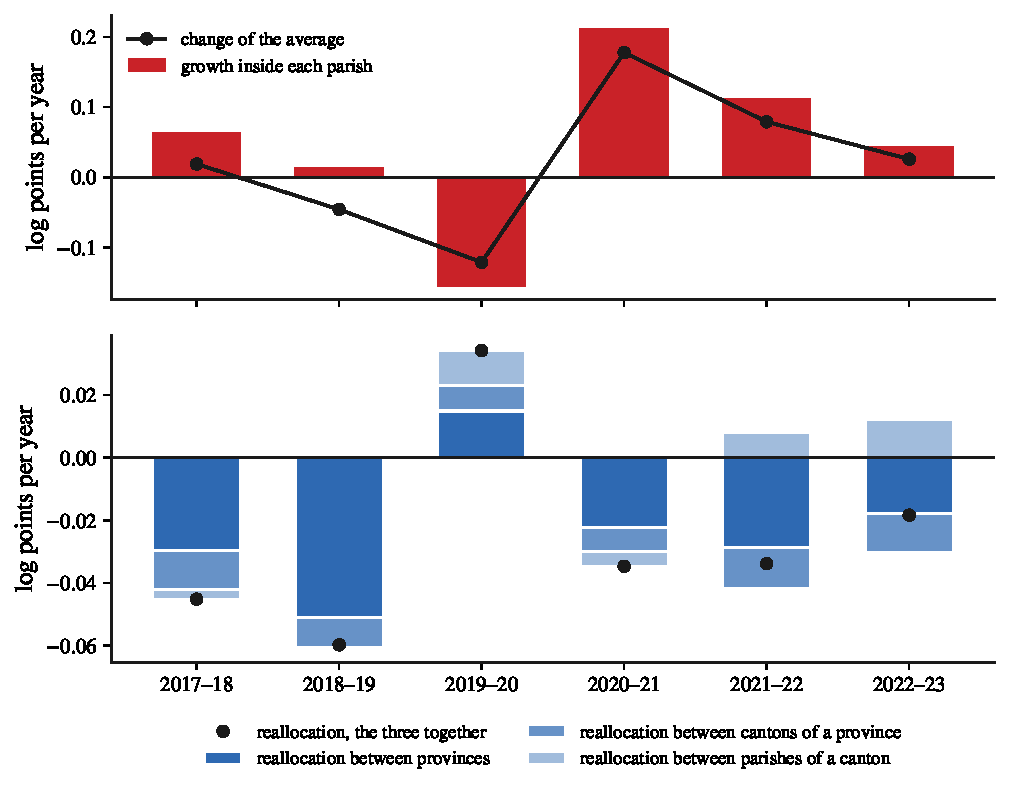
\includegraphics[width=\columnwidth]{change_by_year.pdf}
\caption{The year-by-year decomposition, population path (log points per
year). Top: growth inside each parish (transmission, bars) and the change
of the national average (line). Bottom: selection split by scale (stacked
bars) and its total (dot). The two panels have different vertical axes,
because transmission is several times larger than selection. Only in
2019$\to$2020 are all three components of selection positive.}
\label{fig:byyear}
\end{figure}
% source: results/decomposition/yearly_consecutive_2017_2023/summary_figures/change_by_year.pdf

\subsection{What the selection term is made of}

The trait partition of Section~III answers a question the figure of
$-0.0270$ leaves open: whether firms form in \textit{small} places or in
places where firms \textit{sell little}. The two are easily confused,
because across the 804 parishes log total sales and log firm count have a
firm-weighted correlation of $0.97$. Table~\ref{tab:split} separates the
two parts; each cell of the first row is the exact sum of the two below
it. Size accounts for 88 percent of selection ($-0.0238$ of $-0.0270$):
firm counts grow faster where there are fewer firms, a departure from
Gibrat's law. Only $-0.0032$ belongs to sales per firm, and that
component is not stable: it is negative in four of six annual steps and
positive in 2019$\to$2020 and 2022$\to$2023. The headline therefore reads
as firms dispersing toward smaller places, not toward places where firms
sell less. The size part is spread between provinces ($-0.0174$) and
between cantons ($-0.0096$); the per-firm part exists only between
provinces ($-0.0054$) and is essentially zero within them.

\begin{table}[h!]
\caption{The population-path trait split, 2017--2023 (per year). The
first row is the headline; the other two divide it exactly by
$\ln y_k = \ln n_k + \ln (y_k/n_k)$.}
\label{tab:split}
\centering
\footnotesize
\setlength{\tabcolsep}{1.6pt}
\begin{tabular}{lrrrrrr}
\toprule
Trait & Total & Sel. & \multicolumn{3}{c}{of which} & Transm. \\
\cmidrule(lr){4-6}
 & $\gamma$ & $S$ & prov. & canton & parish & $T$ \\
\midrule
$\ln y_k$      & $+0.0226$ & $-0.0270$ & $-0.0227$ & $-0.0086$ & $+0.0043$ & $+0.0496$ \\
$\ln n_k$      & $+0.0707$ & $-0.0238$ & $-0.0174$ & $-0.0096$ & $+0.0031$ & $+0.0946$ \\
$\ln (y_k/n_k)$ & $-0.0481$ & $-0.0032$ & $-0.0054$ & $+0.0010$ & $+0.0012$ & $-0.0449$ \\
\bottomrule
\end{tabular}
\end{table}

The third row carries a result of its own. The firm-weighted mean of log
sales per firm fell $0.0481$ per year, and that fall is almost all
transmission ($-0.0449$) and very little selection ($-0.0032$): the
decline in sales per firm of Section~IV happened inside places, the two
metropolitan areas included, and not because firms shifted toward places
with lower sales per firm.

\begin{figure}[h!]
\centering
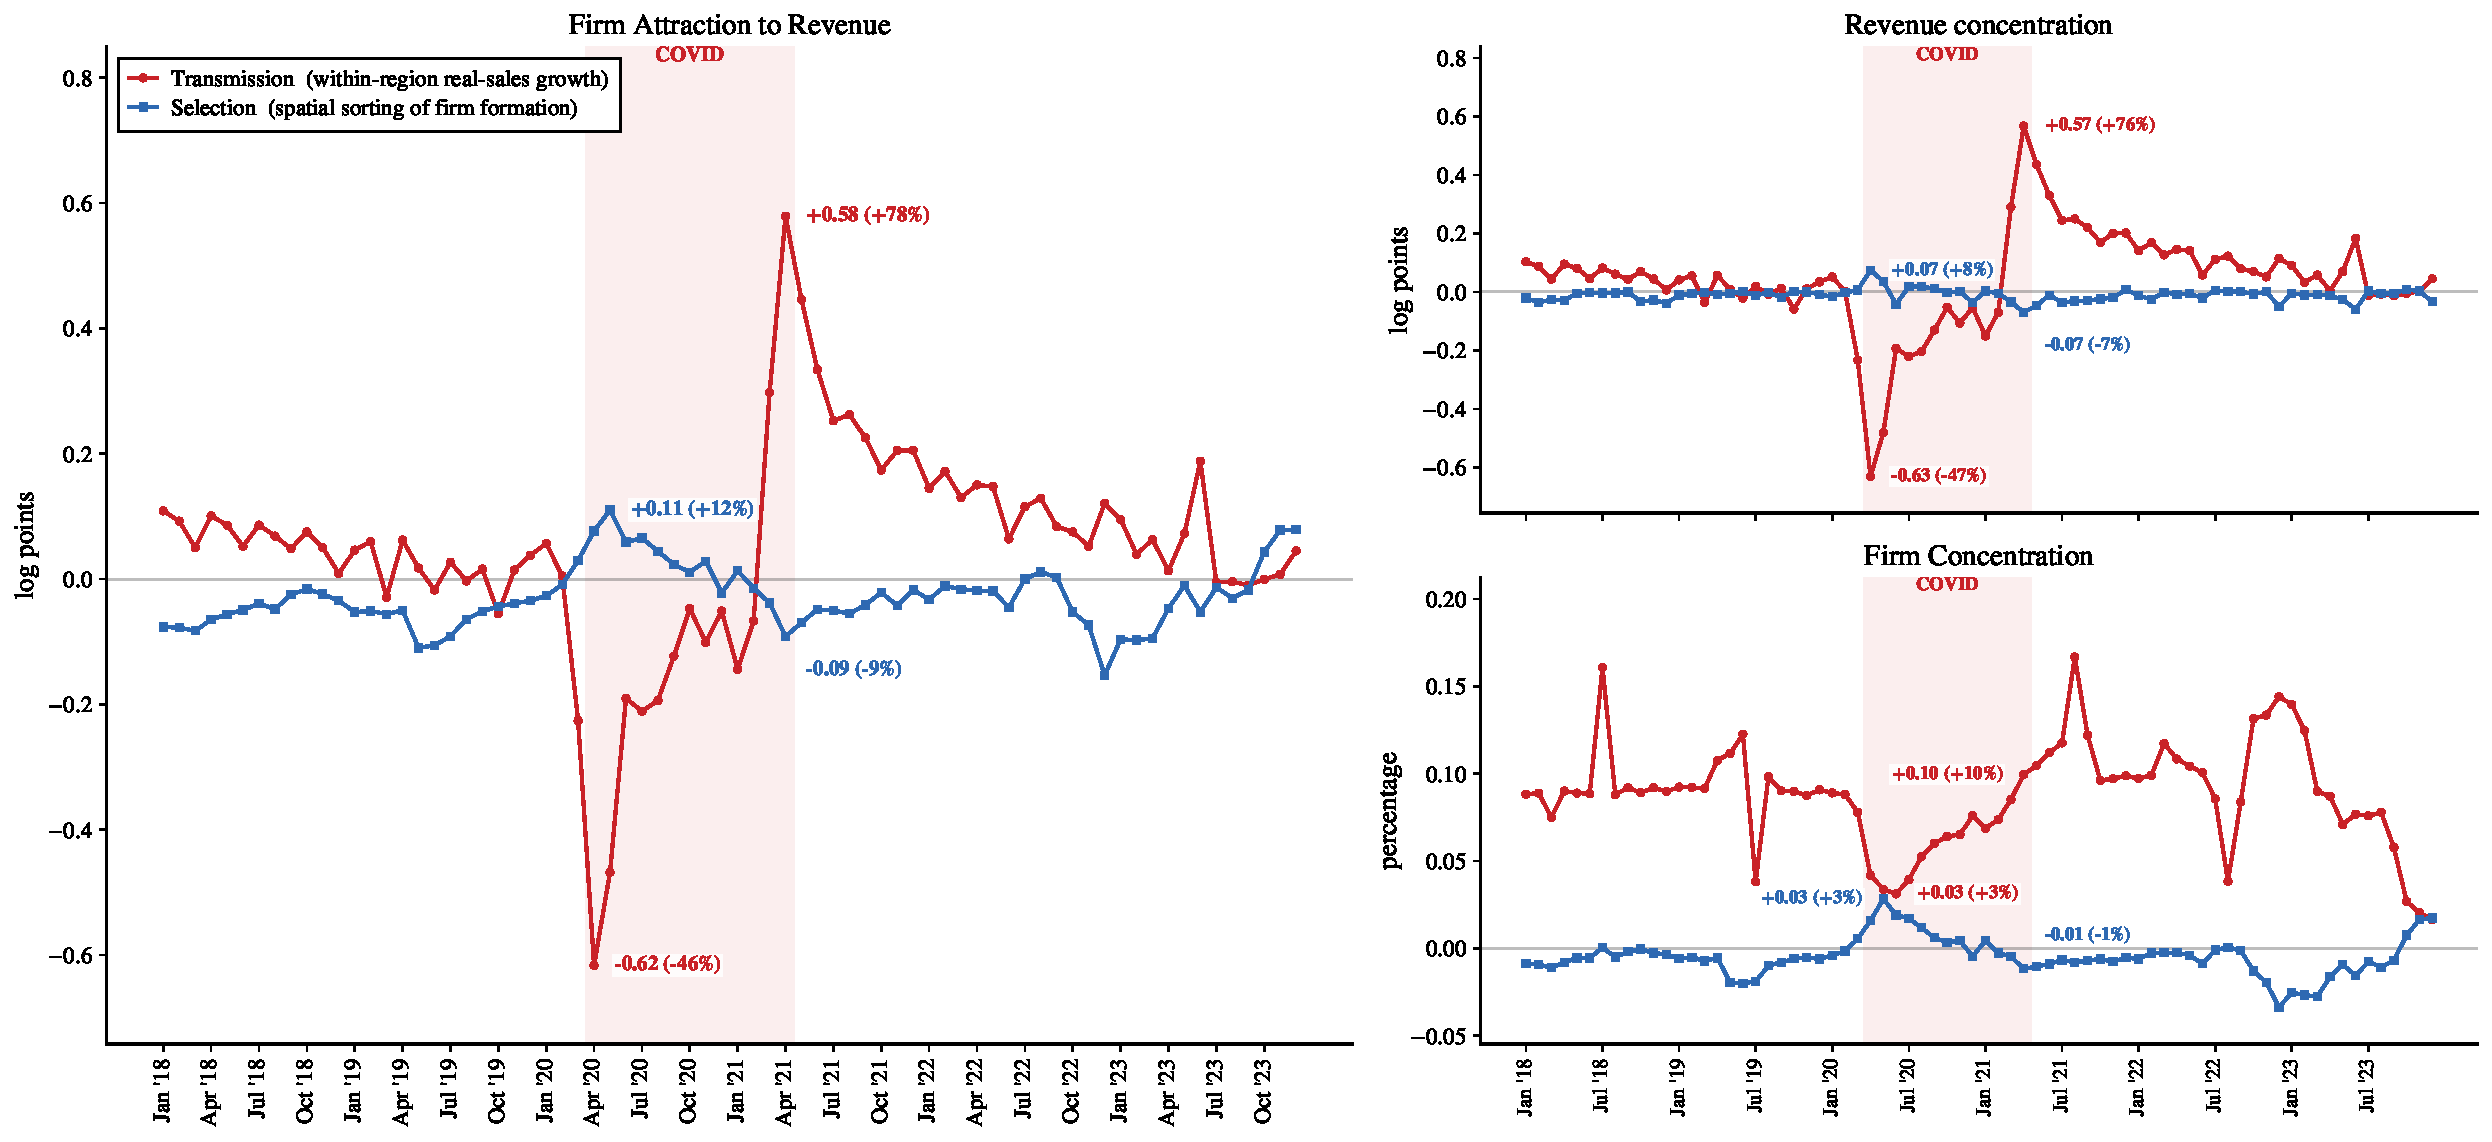
\includegraphics[width=\columnwidth]{monthly_timeseries_all_paths.pdf}
\caption{Selection and transmission on all three paths across 72 rolling
twelve-month windows. All three selection series are negative in normal
times; transmission collapses to $-0.62$ (annualized, $-46$ percent year
over year) in the window ending April 2020 while selection turns
positive.}
\label{fig:monthly}
\end{figure}
% source: results/decomposition/monthly_rolling12_2017_2023/plots/monthly_timeseries_all_paths.pdf
\newpage

\subsection{Three rebalancings, one signature}

Table~\ref{tab:threepaths} and Fig.~\ref{fig:monthly} run the same
question through all three paths. The qualitative claims survive every
rebalancing: selection negative and dominated by the between-province
scale, transmission positive and larger, one reversal in the
2019$\to$2020 step. The magnitudes, however, are not comparable across
paths, because each weights parishes differently: the population path
weights them by firm share, while the income and density paths weight
them by that share times the level, so almost all of their weight falls
on Quito and Guayaquil (Section~III). Income- and density-path selection
should therefore be read as a contrast between the two metropolitan areas
and the rest: their negative sign says that the sales and the firm stock
of Quito and Guayaquil grew more slowly than those of the firm-weighted
average parish. Because density-path selection would be exactly zero
under Gibrat's law, its persistently negative value---five of six years,
through every quarterly lens---rejects proportional growth in favor of
periphery-tilted growth; the size part of Table~\ref{tab:split} is the
same test in logs, not dominated by two parishes and exact at every
scale, and it reaches the same conclusion.

\begin{figure}[h!]
\centering
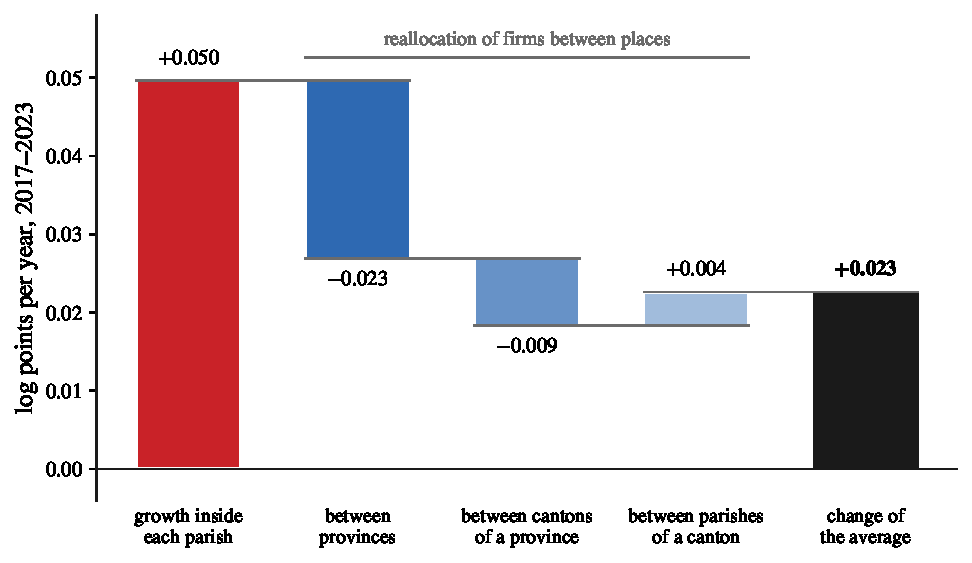
\includegraphics[width=\columnwidth]{change_waterfall.pdf}
\caption{Where the change of the national average comes from, population
path, 2017--2023 (log points per year). Each bar starts where the
previous one ended: growth inside each parish (transmission, $+0.050$),
then the three components of selection, between provinces ($-0.023$),
among cantons of a province ($-0.009$) and among parishes of a canton
($+0.004$); the last bar is the total ($+0.023$).}
\label{fig:waterfall}
\end{figure}
% source: results/decomposition/yearly_consecutive_2017_2023/summary_figures/change_waterfall.pdf

\subsection{The scale anatomy}

The multiscale split \eqref{eq:multiscale} localizes the dispersion
(Table~\ref{tab:threepaths}; Fig.~\ref{fig:waterfall} for the population
path), and none of the
three components is zero. The largest is the \textit{between-province}
term: $-0.0227$ of $-0.0270$, 84 percent, negative in five of six annual
steps. The second, selection \textit{among cantons within provinces}, is
$-0.0086$ per year, a third of total selection (the shares exceed 100
percent because the third component has the opposite sign); it is smaller
but not negligible, with the same sign in the five normal steps. The
third, selection \textit{among parishes within cantons}, is the smallest
($+0.0043$) and the only one of changing sign: positive in 2019$\to$2020
and in the last two steps, when higher-sales parishes (generally cantonal
seats) added firms somewhat faster than their peripheries. It is also the
one scale on which the three paths disagree in sign, so its reading is
the most provisional. Written in percent of national growth, the
population-path cells read $+18.8$, $-37.9$, $-100.4$, $+219.5$---summing
to 100 exactly: within-parish growth delivered 2.2 times the realized
national change, and between-province selection alone gave back an amount
equal to the entire national change.

\begin{figure}[h!]
\centering
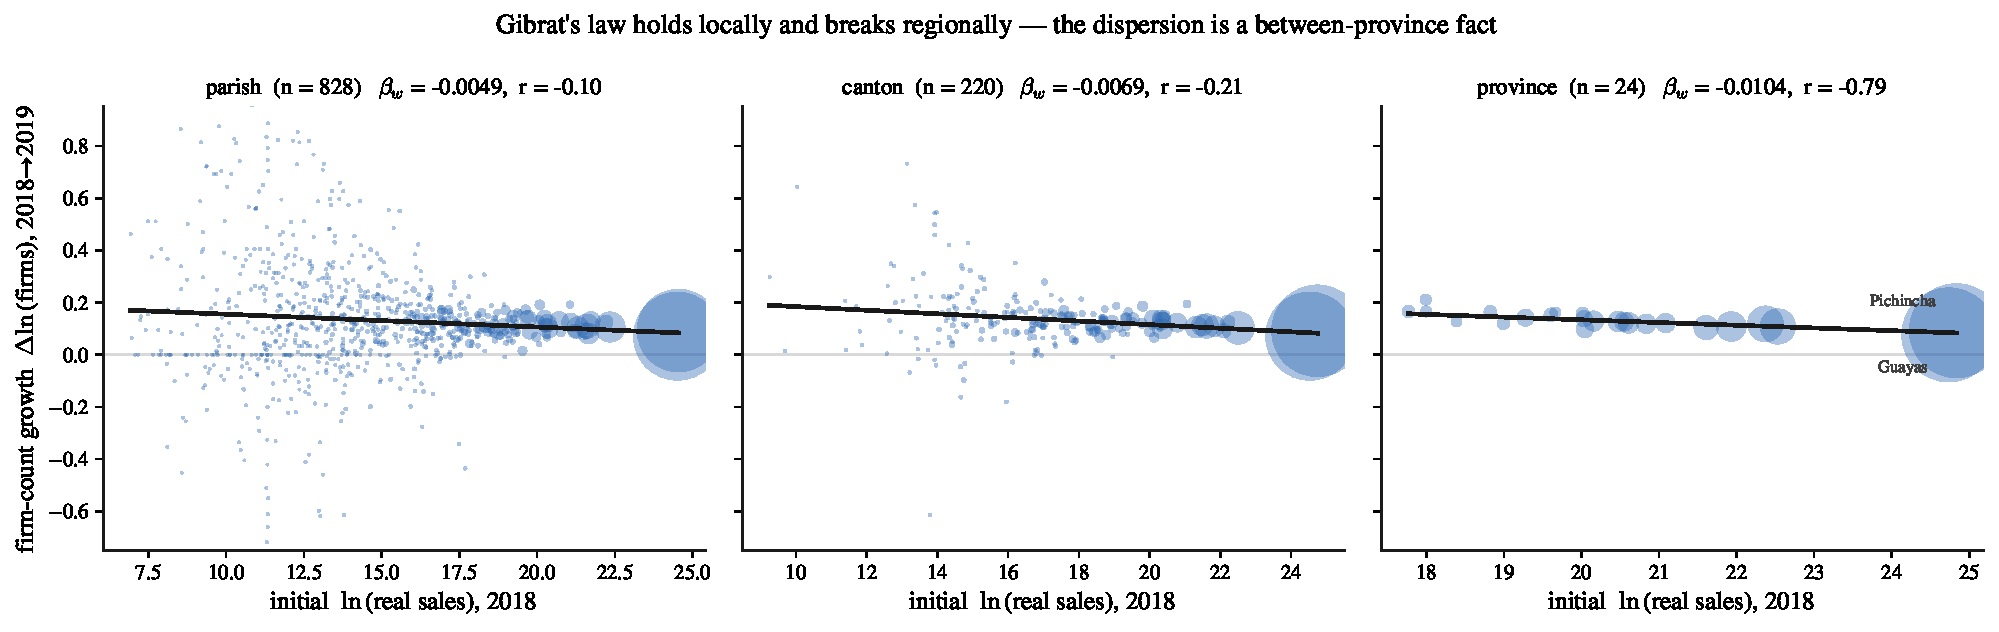
\includegraphics[width=\columnwidth]{scale_scatters.pdf}
\caption{Firm-count growth against initial log real sales at the three
nested tiers (2018$\to$2019). The cloud tilts little at parish and canton
scale and decisively between provinces: Gibrat's law holds approximately
locally and breaks regionally.}
\label{fig:scales}
\end{figure}
% source: results/story/fig2_scale_scatters.pdf

Fig.~\ref{fig:scales} shows the same fact in the raw data: the
growth--size cloud tilts at all three levels, but with very different
slopes. In 2018$\to$2019 the weighted correlation between growth and size
is $-0.10$ among parishes, $-0.21$ among cantons and $-0.79$ among
provinces. Ecuador's firm dynamics are \textit{nearly} scale-free
locally, with a weak tilt of the same sign among cantons, and clearly
converging regionally. A single-scale growth regression pooled across
parishes would report a small departure from Gibrat's law and understate
the effect, because most of the signal lives one or two aggregation
levels up. The speed of the process can be read directly from the shares:
between 2017 and 2023 the part of the firm stock located in Quito and
Guayaquil went from 56.5 to 52.9 percent, 3.5 percentage points in six
years. Spatial deconcentration is real, and it is slow.
\subsection{Who carries the effect}

Decomposing the between-province term by \eqref{eq:contribution} shows a
pincer movement. From the top: Guayas holds 34 percent of firms, sits
$+1.76$ log points above the mean trait, and grew its firm stock 5.4
percent slower than the national average---one quarter of the entire
between-province term from one province. From the bottom: Amazonian
provinces such as Morona Santiago (0.4 percent of firms, $6.9$ log points
below the mean, firm growth 34 percent above average) push the same
covariance negative from below. Influence is concentrated---the single
largest parish contribution (central Guayaquil) is 19 percent of the
summed absolute contributions---but it is concentrated in the economic
centers themselves, whose leverage comes from firm \textit{share}, not from
extreme growth rates; the most explosive parish in the country (a Morona
Santiago parish that went from 8 to 101 firms) contributes almost nothing
because its weight is $7 \times 10^{-5}$. Section~IX makes this
distinction rigorous.

% ============================================================================
\section{The 2019--2020 Inversion}
% ============================================================================

\begin{figure}[h!]
\centering
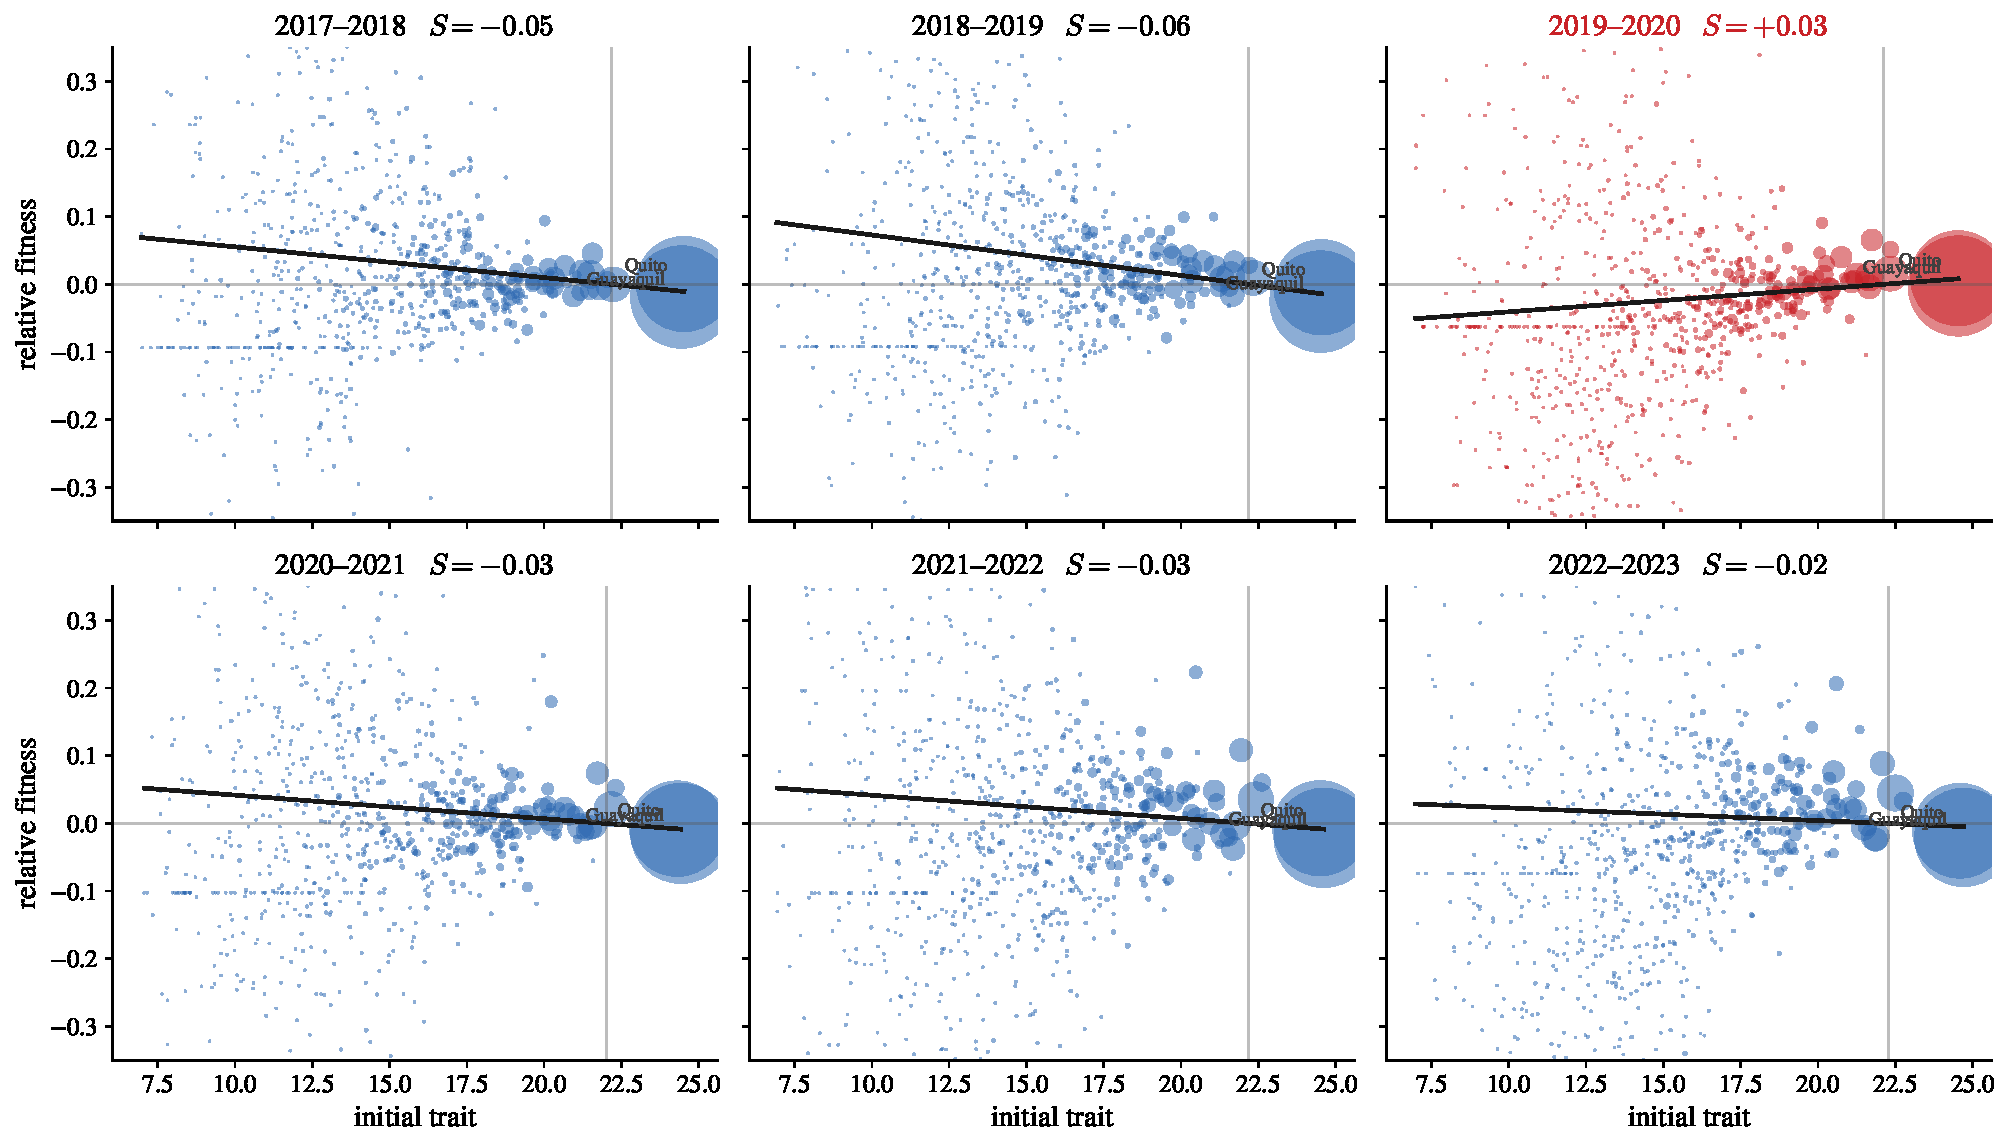
\includegraphics[width=\columnwidth]{selection_flip_scatter.pdf}
\caption{Selection as a tilt, one panel per annual step. Each dot is a
parish at (initial log real sales, relative firm-count fitness), area
proportional to firm share; the line is the firm-share-weighted
regression, whose slope times the trait variance \textit{is} the selection
term. Every normal year tilts down; 2019$\to$2020 tilts up.}
\label{fig:tilt}
\end{figure}
% source: results/selection_anatomy/selection_flip_scatter.pdf

\subsection{The flip, drawn rather than inferred}

The 2019$\to$2020 step coincides with the COVID-19 pandemic and the
lockdown of March--June 2020. This section describes how that step
differed from the others and who carried the difference; it does not
attribute the difference to the pandemic. Selection flips to $+0.0342$
while transmission collapses to $-0.1552$ (Table~\ref{tab:annual}), and
the inversion appears at all three scales at once: $+0.015$ between
provinces, $+0.008$ among cantons within provinces, $+0.011$ among
parishes within cantons. It also appears in both parts of the trait:
$+0.0233$ in the size part and $+0.0109$ in the per-firm part. Because
selection is exactly the tilt of the fitness--trait cloud,
Fig.~\ref{fig:tilt} shows the reversal in the raw data rather than in a
coefficient: the slope runs $-0.045$, $-0.060$, then $+0.034$ in the
pandemic panel, then $-0.035$, $-0.034$, $-0.018$. National growth of
the stock slowed (6.7 percent, against 8.0 to 11.5 percent in the other
steps), the swarm of small low-sales parishes fell below the new bar, and
the metros held just above it---a brief re-concentration. One year later
transmission was the largest in the sample ($+0.2124$).

This result refers to the population of the study, corporations in
activities with reported sales. The same calculation on the complete
registry of active corporations, including those in cells with no
declaration, which is a different object of study, gives a selection of
$-0.0021$ in 2019$\to$2020 (against $+0.0342$) and $-0.0003$ in
2020$\to$2021 (against $-0.0346$). The counts show where the difference
between the two objects comes from. Between 2019 and 2020 the stock of all active corporations grew almost
equally in every
parish size class: 8.1 percent in parishes with fewer than ten
corporations, 7.4 in those with ten to fifty, 6.7 in those with fifty to
five hundred and 7.4 in the larger ones. The stock in cells with reported
sales grew 0.1, 1.1, 5.1 and 7.4 percent, because in small parishes a
larger share of active corporations sat in cells where none reported
sales (from 54 to 60 percent in the smallest class, from 26 to 30 in the
next). The inversion therefore does not describe corporations closing in
the periphery or moving to the cores: the stock of active corporations kept growing at the
same pace everywhere, and what concentrated was activity with reported
sales. In neither object did dispersion continue in 2019--2021: it inverted in
the population with reported activity and stopped in the registry. The
positive sign of selection in that step is therefore a result about
activity with reported sales, not about the registry, and the anatomy
below describes that population.

Two alternative descriptions do not hold in the data. Proximity does not
organize the inversion: a distance-to-hub gradient across parishes is
statistically null overall, surviving only as a faint within-province
tilt explaining about 1 percent of variance---the variable associated
with a parish's outcome was its own size, not its distance to a metro.
Nor is the flip an outlier artifact: it is carried by hundreds of
ordinary parishes, and the unweighted cross-parish distributions are
unchanged when Quito and Guayaquil are removed.

\begin{figure}[h!]
\centering
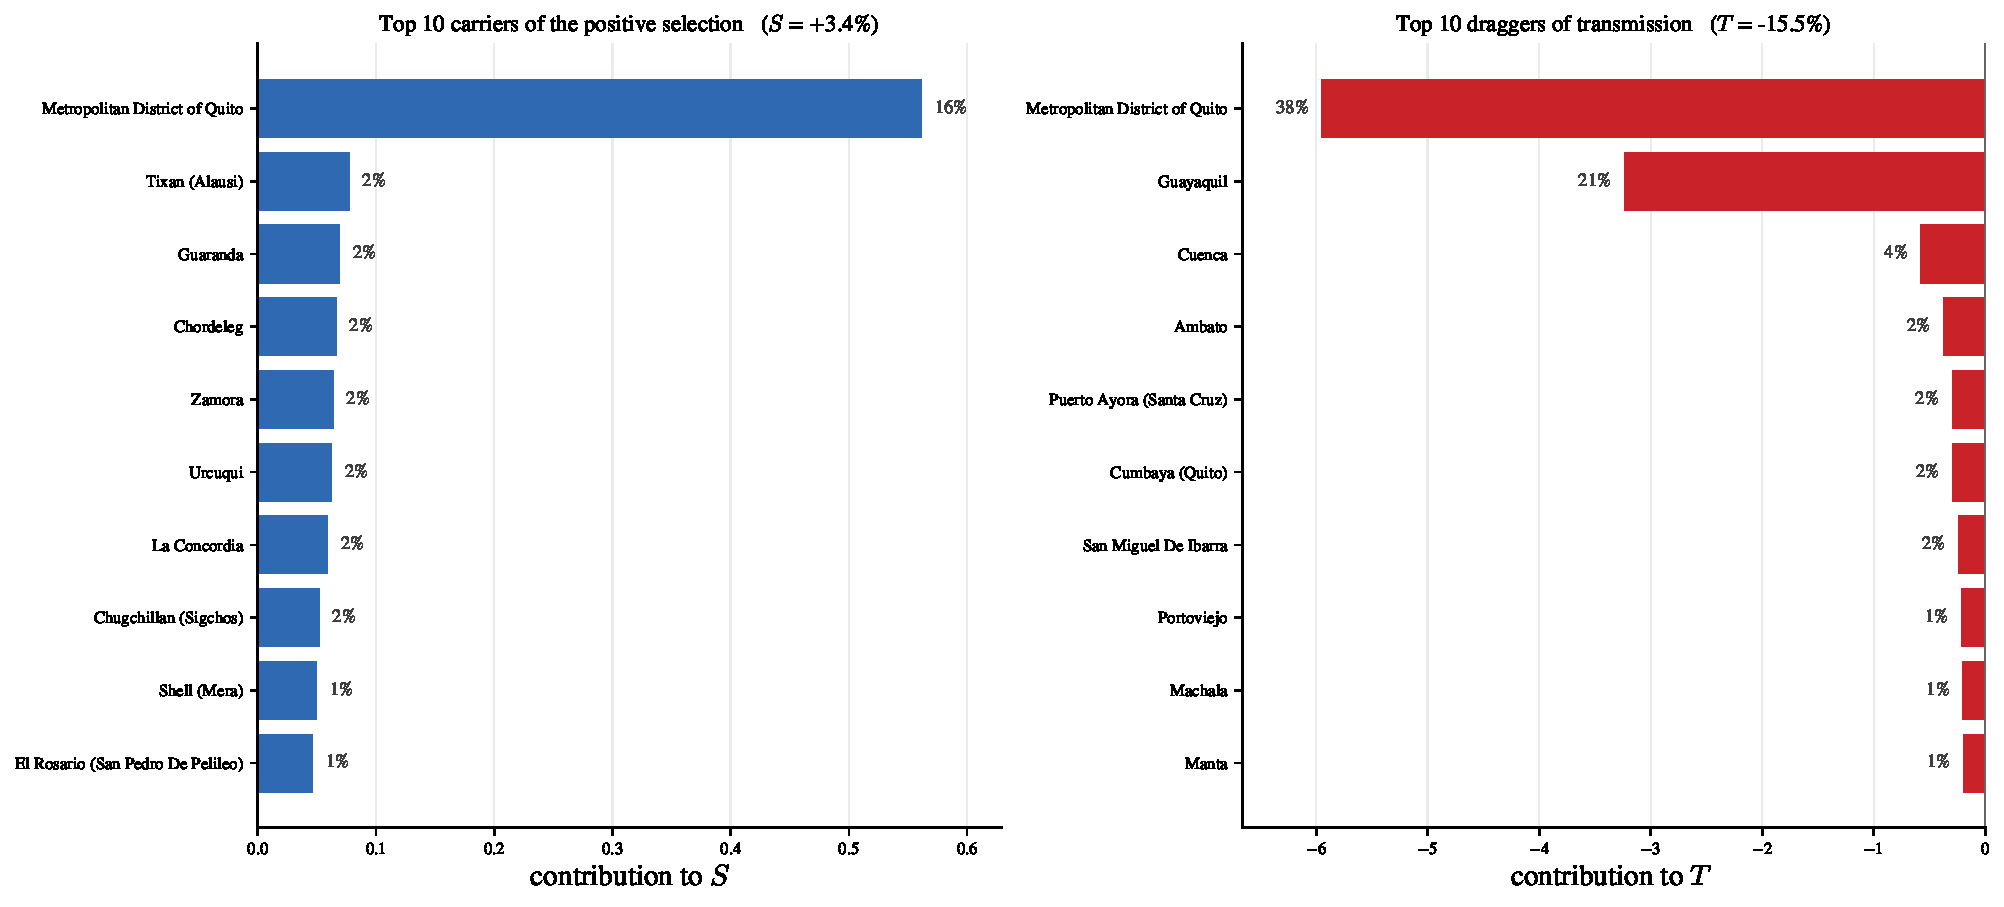
\includegraphics[width=\columnwidth]{covid_carriers_bars.pdf}
\caption{Largest parish contributions to the 2019$\to$2020 selection
(top) and transmission (bottom) terms. Quito is simultaneously the
largest positive selection carrier and the largest transmission
dragger.}
\label{fig:carriers}
\end{figure}
% source: results/selection_anatomy/covid_carriers_bars.pdf

\subsection{What was different about Quito}

Fig.~\ref{fig:carriers} names the carriers, and one city tops both
lists. Quito is the single largest positive selection contributor
($+0.56$ percent per year, 16.4 percent of the entire term) \textit{and}
the single largest transmission dragger ($-5.95$ percent per year, 38.3
percent of that term, with Guayaquil second at 20.9 percent). Through the
COVID step Quito kept adding firms faster than anywhere in the country
($+7.65$ log points against Guayaquil's $+6.43$ and a firm-weighted
national $+6.7$) while its own sales fell furthest among the metros
($-0.22$ against Guayaquil's $-0.11$ in logs). Inside one city, the
extensive and intensive margins came apart.

\begin{figure}[h!]
\centering
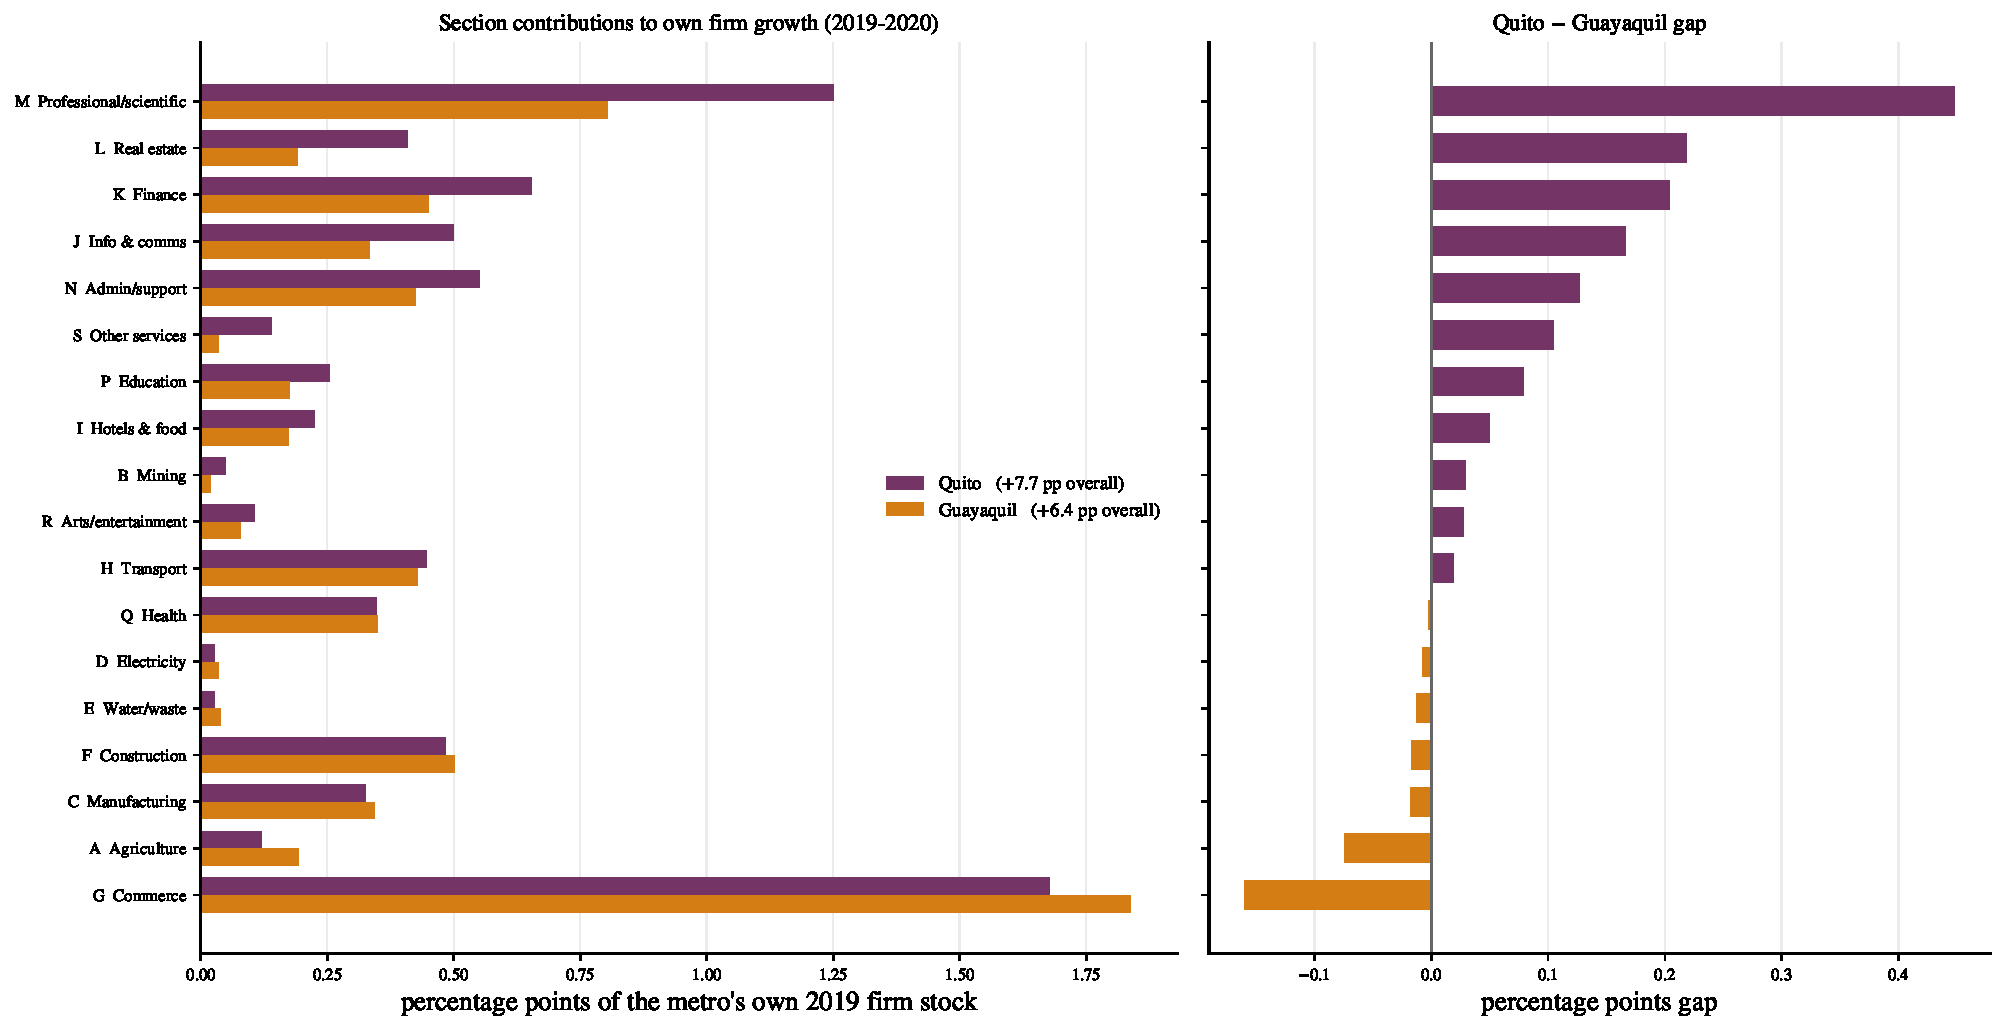
\includegraphics[width=\columnwidth]{metro_sector_contributions.pdf}
\caption{Sector contributions to firm-stock growth through the COVID
step, Quito vs.\ Guayaquil, with the gap by sector. The capital's edge is
concentrated in teleworkable services; commerce, the largest contributor
in both cities, is identical.}
\label{fig:sectors}
\end{figure}
% source: results/selection_anatomy/metro_sector_contributions.pdf

The 1.22-point gap has an address in activity space
(Fig.~\ref{fig:sectors}): professional and scientific services alone
contribute $+0.45$ of it, followed by finance, real estate, information,
and administrative support---teleworkable services, every one. The
control is commerce, the largest contributor in both cities, which grew
at an identical pace ($+1.7$ vs.\ $+1.8$); so the capital's advantage is
associated with its sectoral composition rather than with its size or a
general urban trait. One hypothesis consistent with this pattern is that
Quito's professional-services ecosystem offered a registration margin
that a port-and-transport economy did not, partly as necessity
entrepreneurship; the data describe the pattern but can neither test
that hypothesis nor rule out others.

The same firm-count geography carries a second, quieter regime change:
in windows ending after October 2022, the parishes-within-canton
component of population-path selection decouples from the scale above it
and turns positive, and on the density path the correlation between
canton-level and parish-level selection inverts from $+0.77$ to $-0.40$,
while the income path shows no break ($+0.57$ to $+0.58$). Both breaking
paths are driven by firm counts and the unbroken one by sales: the
rupture is a statement about where firms locate, not where sales are---
mid-size provincial capitals' core parishes began out-adding their own
peripheries---and running a single decomposition could not have said
which.

% ============================================================================
\section{When the Average Is Not a Description}
% ============================================================================

\subsection{Four regimes inside a flat aggregate}

Selection and transmission each carry a sign per unit, so every parish
falls into one of four regimes: \textit{expansion} (gaining firms and
selling more), \textit{consolidation} (stable firms, rising sales),
\textit{dilution} (more firms chasing fewer dollars), and \textit{abandonment} (losing both). Loja 2023$\to$2024,
the flat aggregate of the introduction, contains all four
simultaneously: its firm-weighted ledger reads
$\Delta \bar z = -0.039 = S\,(-0.049) + T\,(+0.010)$---the environment of
the typical formal firm deteriorated by about four percent inside a
province whose dollar aggregate moved $+0.0$ percent. A dollar-weighted
average---any average---is structurally unable to say that sentence.

\begin{figure}[h!]
\centering
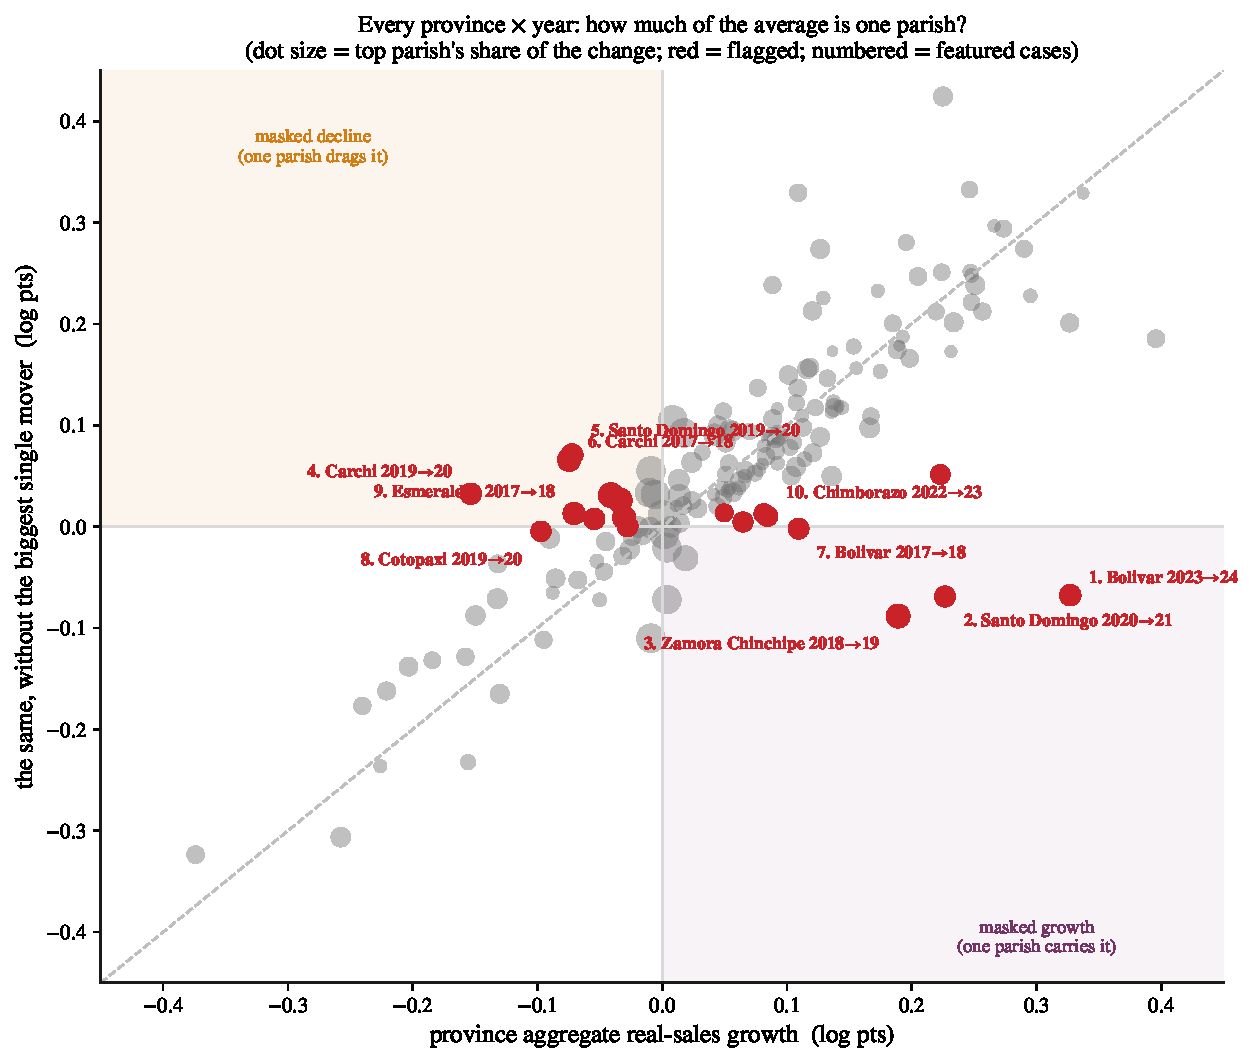
\includegraphics[width=\columnwidth]{masked_scan.pdf}
\caption{Every province $\times$ annual step 2017$\to$2024: aggregate
real-sales growth $G$ against the same growth without the largest single
mover $G_{-1}$. Off-diagonal red points are masked growth (southeast) or
masked decline (northwest); numbered points are the featured cases of
Table~\ref{tab:masked}.}
\label{fig:scan}
\end{figure}
% source: results/story/masked_multiscale/fig0_dashboard_vs_leave_one_out.pdf

\subsection{A three-number audit of any growth figure}

The enclave problem generalizes. Three numbers per (province, window),
all computable from the per-unit ledger the pipeline already exports,
form a detector: the aggregate growth $G = \Delta \ln \sum_k y_k$; the
\textit{leave-one-out} growth $G_{-1}$, dropping the parish with the
largest absolute dollar change; and the median parish growth $\tilde g$.
Masked growth is $G$ clearly positive with $G_{-1} \lesssim 0$ (or the
gap most of $G$); masked decline is the mirror. Scanning all 168
province-years (Fig.~\ref{fig:scan}, Table~\ref{tab:masked}) flags 19:
about one provincial growth number in nine is, to first order, a single
parish.

\begin{table}[h!]
\caption{Masked growth and masked decline, selected cases (all values
percent).}
\label{tab:masked}
\centering
\footnotesize
\setlength{\tabcolsep}{3pt}
\begin{tabular}{llrrrl}
\toprule
Province & Step & $G$ & $G_{-1}$ & $\tilde g$ & carried by \\
\midrule
\multicolumn{6}{l}{\textit{masked growth}}\\
Bol\'ivar        & 23$\to$24 & $+38.7$ & $-6.5$ & $+6.0$  & Guaranda \\
Sto.\ Domingo    & 20$\to$21 & $+25.4$ & $-6.7$ & $+12.3$ & Sto.\ Domingo \\
Zamora Ch.       & 18$\to$19 & $+20.8$ & $-8.4$ & $+25.7$ & Los Encuentros \\
\multicolumn{6}{l}{\textit{masked decline}}\\
Carchi           & 19$\to$20 & $-14.2$ & $+3.3$ & $-13.5$ & Tulc\'an \\
Sto.\ Domingo    & 19$\to$20 & $-7.0$  & $+7.4$ & $-2.7$  & Sto.\ Domingo \\
Tungurahua       & 23$\to$24 & $-5.3$  & $+0.8$ & $-1.2$  & Ambato \\
\bottomrule
\end{tabular}
\end{table}

\begin{figure}[h!]
\centering
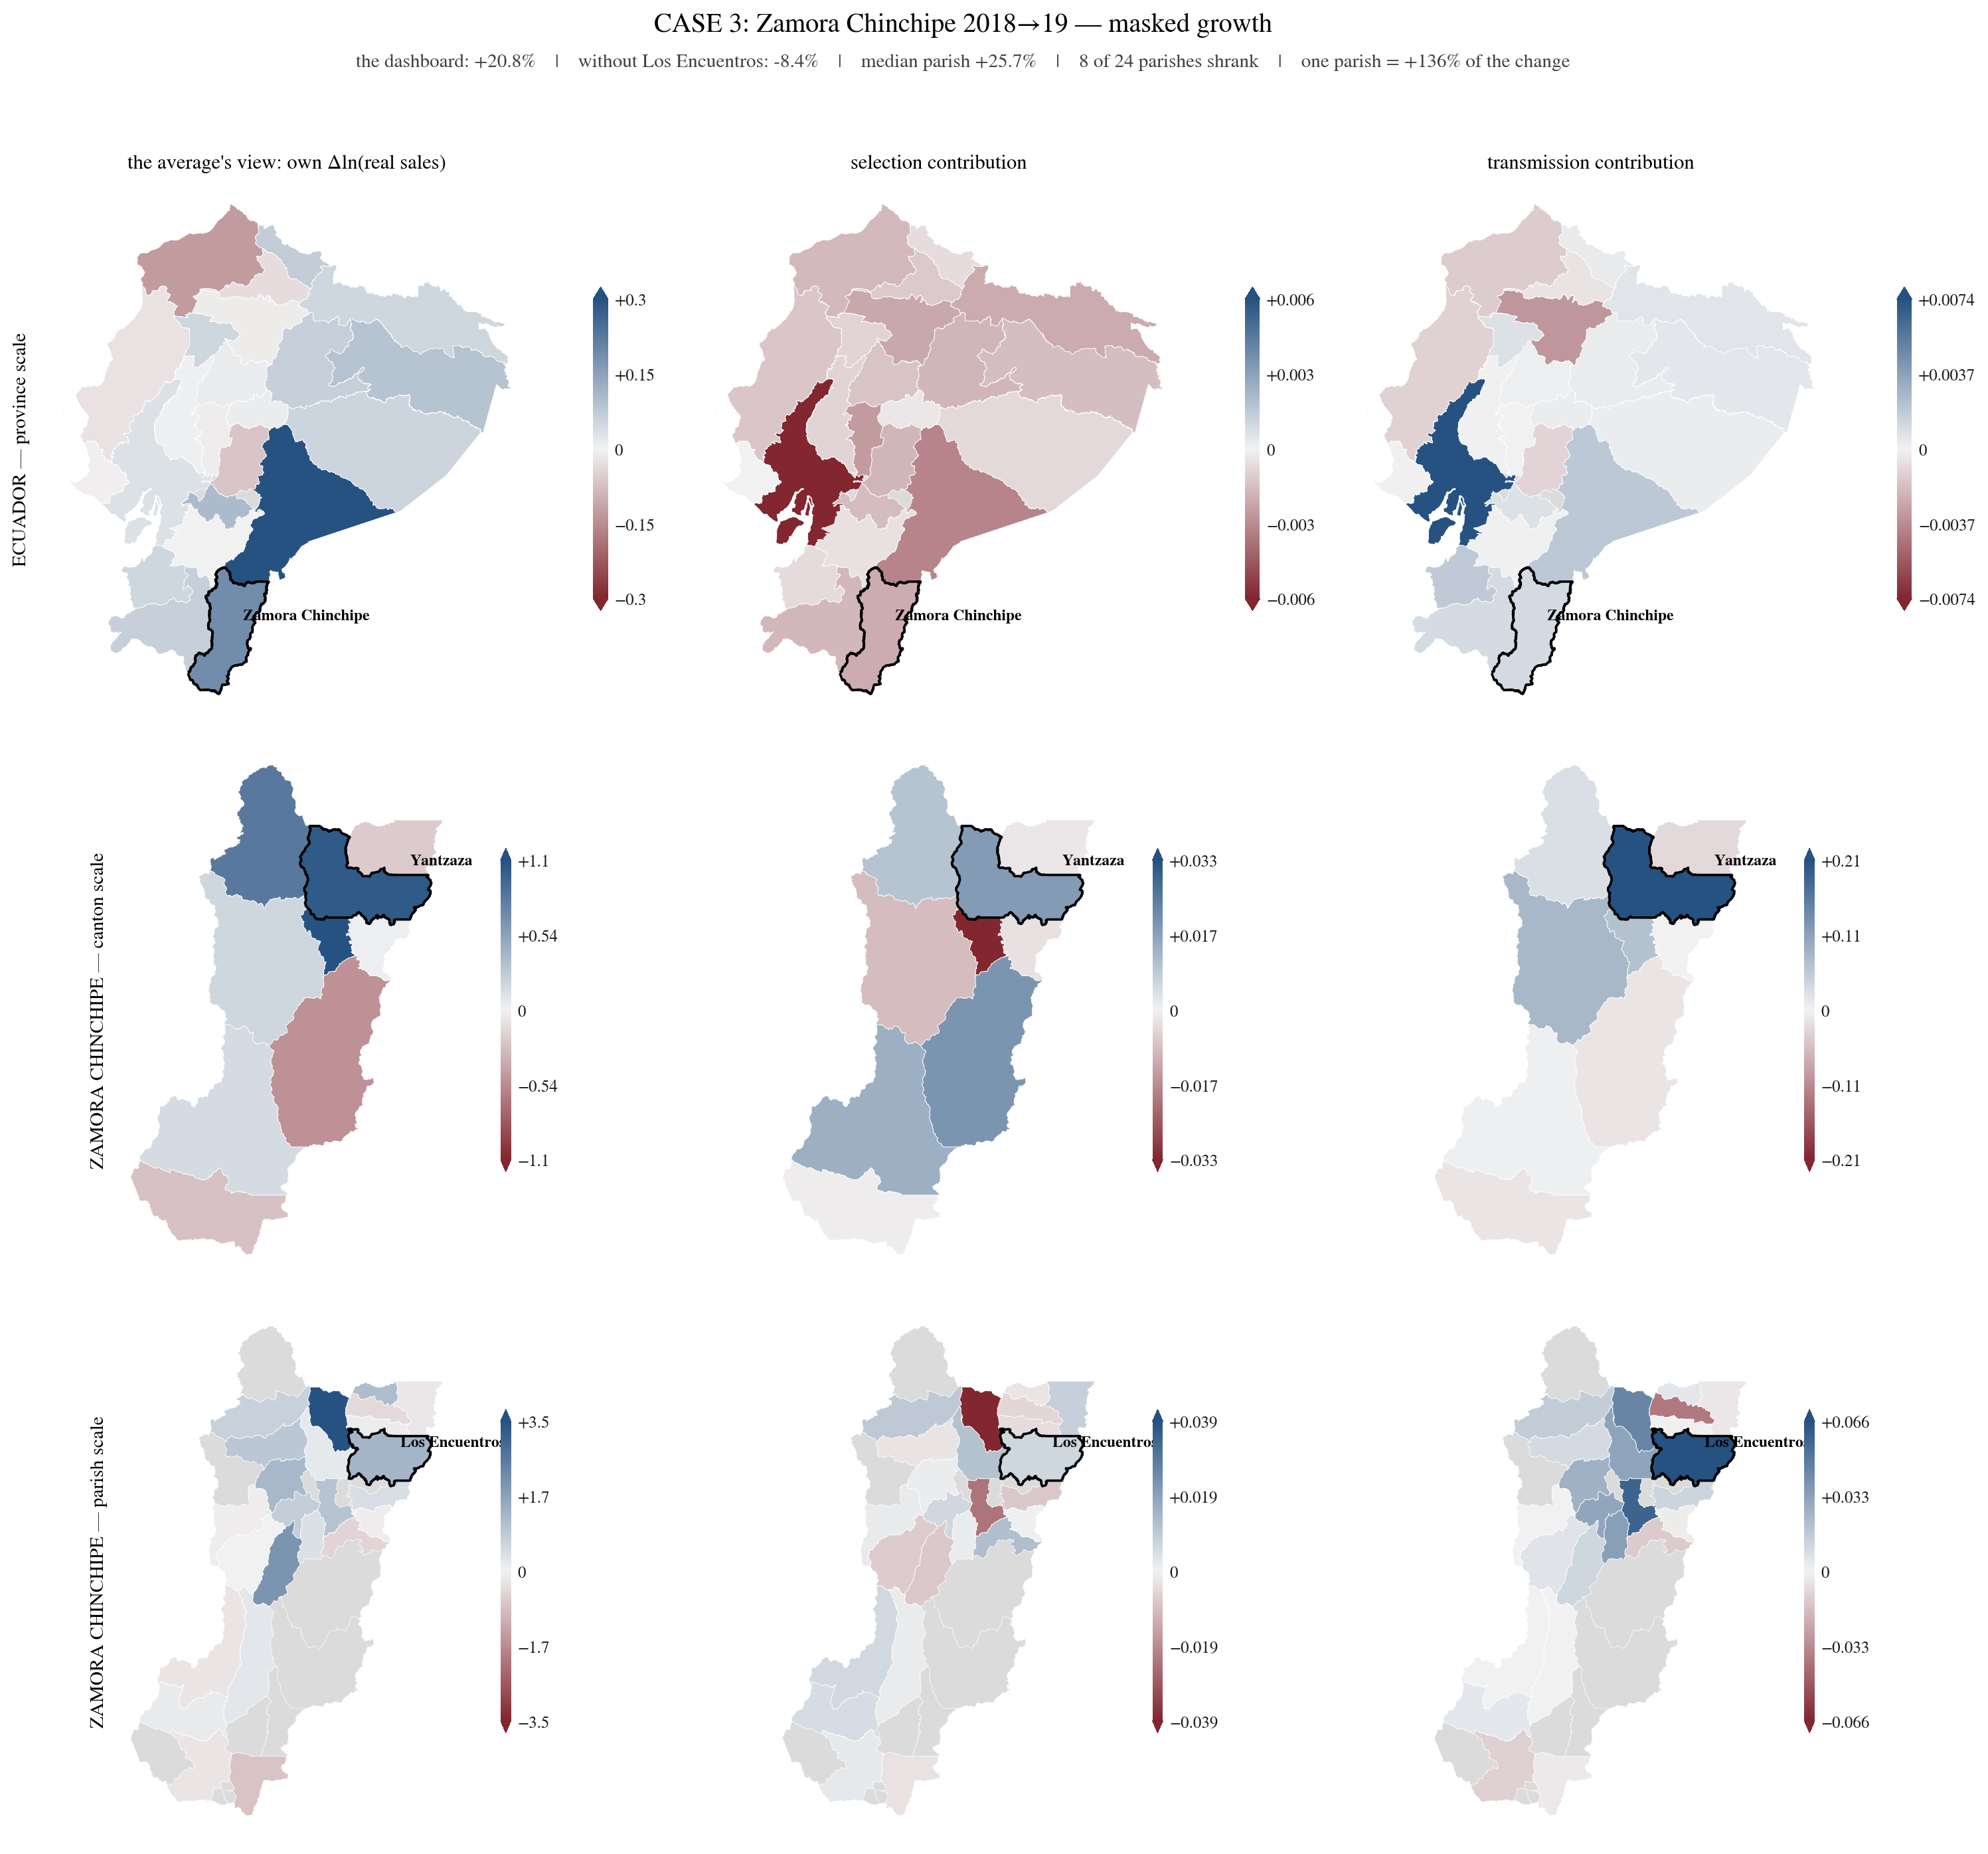
\includegraphics[width=\columnwidth]{case_zamora.png}
\caption{The enclave case at three scales: Zamora Chinchipe 2018$\to$19.
Rows go coarse to fine (country at province scale; the flagged province
at canton and parish scale, with the decomposition re-run within the
province); columns go average to decomposition (own sales growth,
selection contribution, transmission contribution). The national map
shows unremarkable growth; the zoom concentrates the entire transmission
signal in the single parish of Los Encuentros while province-wide
selection is negative.}
\label{fig:zamora}
\end{figure}
% source: results/story/masked_multiscale/case3_19_2018_2019.png
\newpage
The flagship case is Zamora Chinchipe (Fig.~\ref{fig:zamora}), home of
Fruta del Norte, Ecuador's first large-scale gold mine, in the parish of
Los Encuentros: about a dozen formal firms whose real sales went from
\$7.2 million and 7.8 percent of the province in 2017 to \$1.15 billion
and 43 percent of the province in 2024. In 2018$\to$19 the province
``grew'' $+20.8$ percent---but $-8.4$ percent without Los Encuentros,
while the \textit{median} parish grew $+25.7$ percent; in the COVID year
the aggregate grew $+377$ percent while the median parish shrank $-24$
percent. The dollar ledger attributes essentially the whole increase to
one parish; the Price ledger, weighting one-firm-one-vote, barely notices
five firms. \textit{The disagreement of the two ledgers is the enclave
signature}, and the mirror case works identically: Carchi's ``$-14.2$
percent collapse'' in the COVID year is one closed border town (Tulc\'an),
without which the agricultural province \textit{grew} $+3.3$ percent---and
within the province the two Price terms disagree in sign, which is
precisely the audit flag. The masked cases are not data errors---the
mine's sales are real. The error is treating a sum as a description, and
the decomposition's two weightings institutionalize the audit.

% ============================================================================
\section{Does Diversification Buy Resilience?}
% ============================================================================

\begin{figure}[h!]
\centering
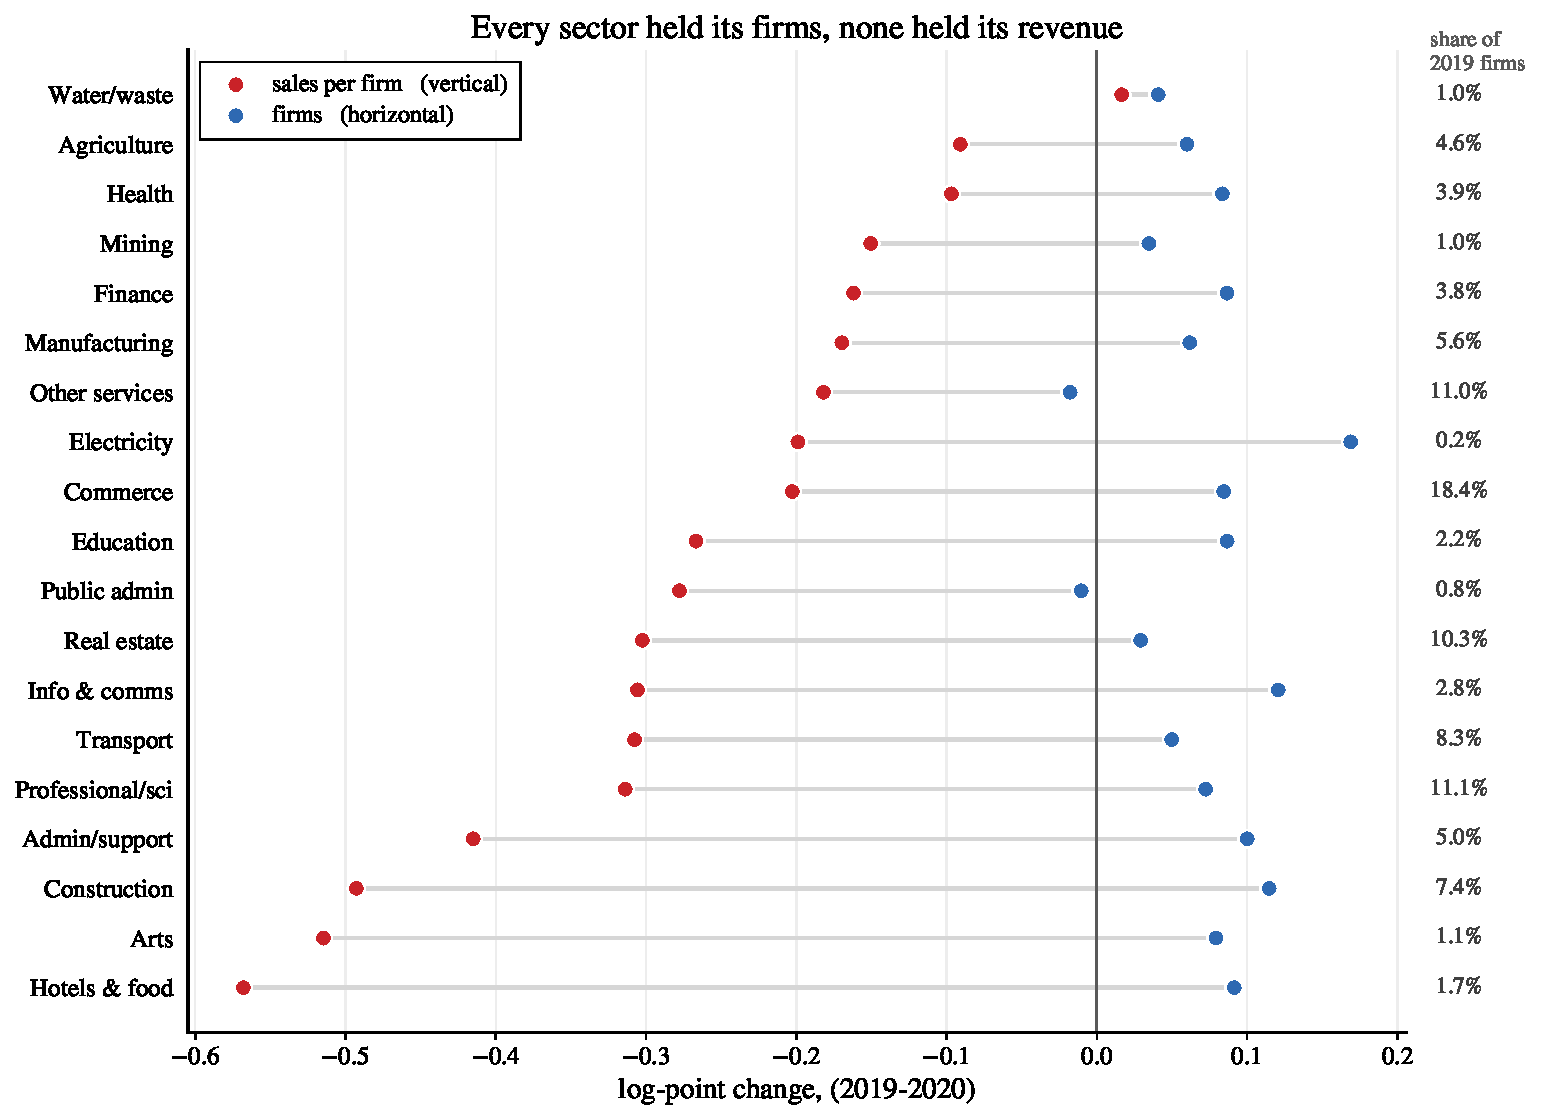
\includegraphics[width=\columnwidth]{sector_margins.pdf}
\caption{The COVID step by sector: change in firm count (extensive) and
in sales per firm (intensive), which sum exactly to sales growth per
\eqref{eq:margins}. Seventeen of nineteen sectors kept adding firms; one
of nineteen held its sales per firm.}
\label{fig:sectormargins}
\end{figure}
% source: results/resilience/regular_economy/fig10_sector_margins.pdf

\subsection{Fragility is a sales phenomenon; resilience is an entry
phenomenon}

Sectorally (Fig.~\ref{fig:sectormargins}), the two margins of
\eqref{eq:margins} split the shock asymmetrically: sales per firm spans
0.58 log points across CIIU sections (accommodation and food $-0.57$,
construction $-0.49$, water $+0.02$) while firm counts span only 0.19,
with 17 of 19 sections still adding firms; across sectors the two margins
correlate at $-0.27$---weak and, if anything, negative. Fragility and
resilience are different traits of the same place: Quito sits
simultaneously at the 28th percentile of sales resistance and the 75th of
firm resistance. One caution applies: the firm count comes from the
registry, where a corporation stays active until it suspends or cancels
its registration, so part of the stability of the extensive margin
reflects that inertia rather than activity.

The concentration that makes places fragile is double. Spatially, the
median province books its formal sales in about four effective parishes
(Pastaza and Santo Domingo hold 88 percent in one parish). Sectorally,
the deepest and longest COVID craters are all one-activity places---
tourism monocultures such as Puerto Villamil ($-2.1$ log points, 45
months under water) and Puerto Ayora ($-2.0$, 39 months)---and exposure
to hard-hit activities predicts the hit (Spearman rank correlation about
$-0.5$, size-partialled). When the shock is correlated, \textit{which}
activities a place holds matters more than how many.

\begin{figure}[h!]
\centering
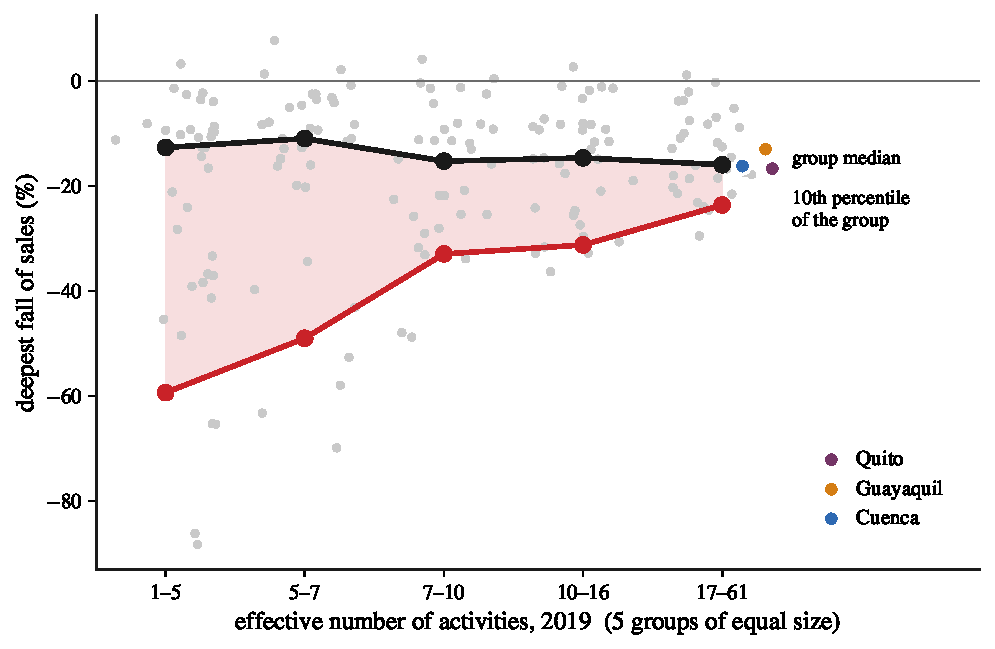
\includegraphics[width=\columnwidth]{breadth_groups.pdf}
\caption{Breadth and the depth of the sales fall across the 174 parishes
with at least 50 firms (oil and mega-cells removed), ordered by breadth
and cut into five groups of equal size. Each dot is a parish; the three
cities are in the broadest group. The black line joins the median fall
of each group, the red line its 10th percentile (the fall only one
parish in ten of the group exceeded). The black line is flat and the red
one rises: the median is similar across groups and the 10th percentile
improves with breadth.}
\label{fig:breadthgroups}
\end{figure}
% source: results/resilience/regular_economy/fig3_breadth_groups.pdf

\subsection{Breadth and the absence of extreme falls}

Measuring a parish's breadth as the effective number of activities
$D = e^{H}$, with $H$ the Shannon entropy over the sales shares of CIIU
rev.~4 activity groups at a frozen 2019 baseline, Fig.~\ref{fig:breadthgroups}
delivers a two-part verdict across the 174 parishes with at least 50
firms. Population and variable are those of the rest of the paper:
private corporations and total sales. As a predictor of the \textit{size}
of the sales trough, breadth does almost nothing: the rank correlation is
$-0.03$ in the full economy and $+0.05$ ($p = 0.49$) once the four oil
activity groups and the mega-cells are removed from both sides. A
mega-cell is a parish $\times$ activity cell whose 2019 sales per
taxpayer exceed the 99th percentile of all cells; the extract documents
only a range of taxpayers per cell, so sales are divided by the top of
that range, which makes the figure a lower bound and the flag
conservative. The 2020 fall was a composition shock: applying to each
parish's 2019 activity mix the change each activity recorded in the rest
of the country reproduces much of the ordering of the observed falls
(rank correlation $+0.53$), and breadth is related neither to the
mix-predicted fall ($-0.08$) nor to the gap between observed and
predicted ($-0.07$; neither significant). Quito is the metro that departs
from its mix: its sales fell 20.3 percent against a predicted 14.7
percent, while Guayaquil and Cuenca fell almost exactly as predicted.
What is observed is that extreme falls are concentrated in narrow
economies: the worst trough among the thirteen parishes with at least 30
effective activities is $-0.27$ log points, against $-2.15$ among the
other 161, and firm-base growth correlates with breadth at $+0.29$
($p = 0.0001$).

\begin{figure}[h!]
\centering
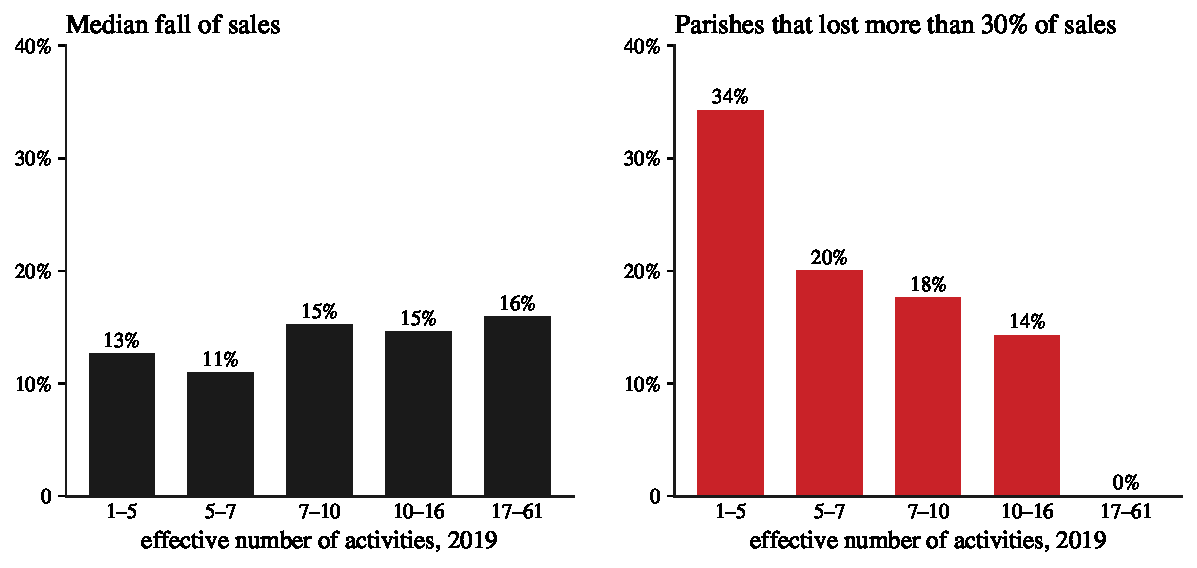
\includegraphics[width=\columnwidth]{typical_vs_severe.pdf}
\caption{The same five groups in two indicators. Left: median fall of sales
(group median). Right: share of the group's parishes that lost more than
30 percent of their sales.}
\label{fig:severe}
\end{figure}
% source: results/resilience/regular_economy/fig9_typical_vs_severe.pdf

\begin{figure}[h!]
\centering
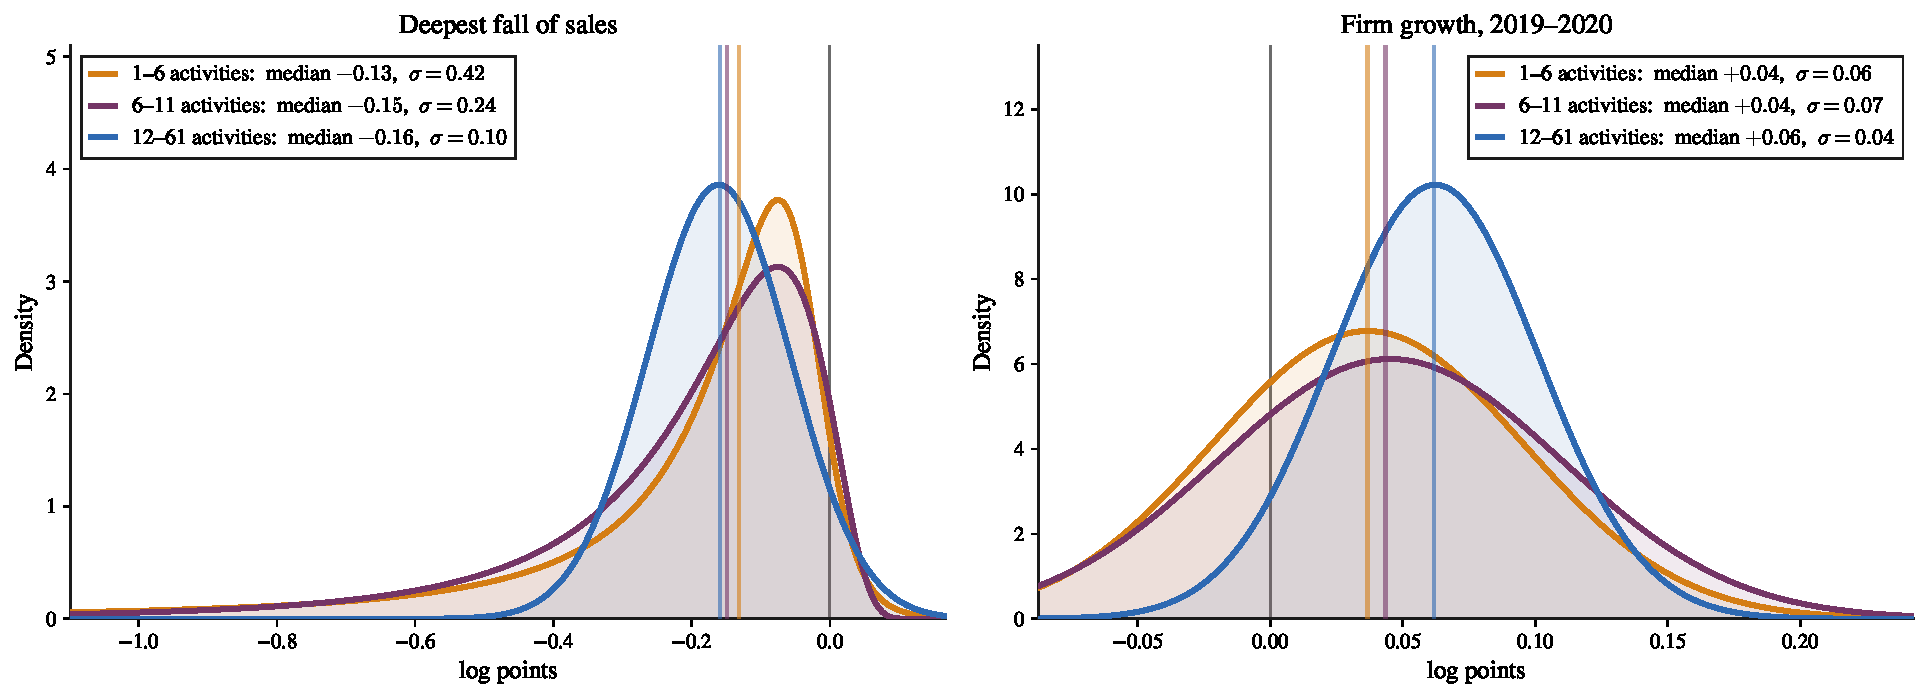
\includegraphics[width=\columnwidth]{breadth_distributions.pdf}
\caption{Fitted distributions, in log points, of the fall of sales (left)
and of firm-count growth in 2019$\to$2020 (right) for the 174 parishes cut
by breadth into three groups of equal size (58 parishes each). Each curve
is a continuous fit (a skewed Student-$t$ when it beats the Gaussian by at
least ten AIC points, otherwise the Gaussian); the vertical line of the
same color marks the group median and $\sigma$ is the standard deviation.
The axes span the 3rd to the 99.5th percentile of each variable, which
leaves out three parishes on the left and four on the right.}
\label{fig:breadthdist}
\end{figure}
% source: results/resilience/regular_economy/fig11_breadth_distributions.pdf

The distributional statement (Figs.~\ref{fig:breadthgroups},
\ref{fig:severe} and~\ref{fig:breadthdist}) is the sharper one. Ordering the 174 parishes by
breadth and cutting them into five groups of equal size, the median fall
of sales is nearly the same in all of them: 13, 11,
15, 15 and 16 percent from the narrowest to the broadest. What changes is
the lower tail. The 10th percentile of each group, the fall that only one in ten of
its parishes exceeded, goes from 59 percent in the narrowest group to 49,
33, 31 and 24 percent, and the share of parishes that lost more than 30
percent of their sales goes from 34 percent to 20, 18, 14 and 0. The
result does not depend on the choice of five groups: a Brown--Forsythe
test rejects equal spreads with two, three, four and five groups ($p$
between $0.0006$ and $0.013$), and with no groups at all a quantile
regression on log breadth has a slope of $+0.171$ ($p = 0.0003$) at the
10th percentile and $-0.020$ ($p = 0.29$) at the median.
Fig.~\ref{fig:breadthdist} shows the whole shape with three groups: the
medians of the fall nearly coincide ($-0.13$, $-0.15$ and $-0.16$ log
points from the narrowest to the broadest), its standard deviation shrinks
from $0.42$ to $0.24$ and $0.10$, and the tail toward large falls, visible
in the two narrower groups, is absent in the broadest. Broader parishes
took, if anything, a somewhat larger hit per firm: the rank correlation
of breadth with the change in sales per firm is $-0.17$ ($p = 0.03$). On
the extensive margin, 97 percent of the parishes in the broadest group
added firms against 74 percent in the narrowest, but the spread of firm
growth does not shrink robustly with breadth ($p = 0.09$ with three
groups, $0.11$ with five), so the statement is about sales only. Breadth
is not associated with a smaller average shock but with the absence of
extreme falls, the pattern the portfolio argument of the regional variety
and resilience literature predicts~\cite{martin2015,frenken2007}.

These data do not allow attributing the pattern to diversification.
Breadth and size move together in Ecuador (correlation $+0.65$). There is
also a mechanical reason to expect the pattern with no diversification
effect at all: the total of a large parish sums thousands of firms whose
individual changes offset each other, so it fluctuates less than the
total of a parish with few firms; and comparing the worst fall of a group
of 13 with that of a group of 161 favors the small group by
construction. Three checks measure what is left after those objections.
(a)~\textit{A permutation test.} Of 20{,}000 random groups of 13
parishes, only 1.4 percent have a worst fall as mild as the broad
group's, so the result is not chance; drawn only from the 39 largest
parishes, the share rises to 4.4 percent, and in the full economy (nine
broad parishes) the two figures are 4.3 and 6.3 percent. Against parishes
of their own size the advantage of broad ones is marginal.
(b)~\textit{Breadth and size in one regression.} With log firms and log
breadth as regressors, neither is associated with the average depth of
the sales trough; at the bad end of the distribution (quantile regression
at the 10th percentile) and in the dispersion of outcomes, breadth keeps
a significant association and size does not. For firm growth it is the
reverse: size goes with less dispersion, and net of size no relation with
breadth remains ($+0.05$). The two variables are strongly correlated, so
these signs are indications, not magnitudes. (c)~\textit{Another
downturn.} Between 2015 and 2016, with the oil-price collapse and the
April 2016 earthquake, real private-corporation sales fell 0.09 log
points. With the same parishes and breadth measured in 2015 the pattern
points the same way (rank correlation $-0.11$, not significant; worst
change $-0.14$ among the seven broad parishes against $-0.86$ in the
rest), but a random group of seven matches it 12.7 percent of the time:
the check neither contradicts nor confirms the 2020 result. The
defensible statement is that, in the fall of sales, broad economies
avoided the worst outcomes, an advantage that narrows to a thin margin
against parishes of their own size; for the number of firms, what counts
is size. The result is an association, not a mechanism, and it remains
preliminary.

% ============================================================================
\section{Robustness}
% ============================================================================

\begin{table}[!t]
\caption{The outlier trial: full-window population-path selection under
outlier treatments and data-validity floors.}
\label{tab:robust}
\centering
\small
\begin{tabular}{lrrr}
\toprule
Variant & $S^{p}$ & btw.\ prov. & $T^{p}$ \\
\midrule
raw                   & $-0.0270$ & $-0.0227$ & $+0.0496$ \\
winsorized p1/p99     & $-0.0265$ & $-0.0224$ & $+0.0494$ \\
trimmed p1/p99        & $-0.0262$ & $-0.0221$ & $+0.0492$ \\
\midrule
floor \$1 (859 par.)     & $-0.0263$ & $-0.0228$ & $+0.0501$ \\
floor \$1{,}000 (804)    & $-0.0270$ & $-0.0227$ & $+0.0496$ \\
floor \$100{,}000 (576)  & $-0.0276$ & $-0.0223$ & $+0.0485$ \\
\bottomrule
\end{tabular}
\end{table}

Selection is a covariance between a mild variable and a wild one: the
trait has skew $+0.14$ and excess kurtosis $-0.44$, while the raw fitness
ratio has skew $+5.0$, kurtosis $+45$, and a maximum of $17.6\times$. A
variable that heavy-tailed could, in principle, let a few explosive
parishes dictate the headline. It does not (Table~\ref{tab:robust}):
winsorizing or trimming fitness at its 1st/99th percentiles moves
selection by less than 3 percent, and sweeping the data-validity floor
from \$1 to \$100{,}000 per year---the last step dropping a third of all
parishes---leaves full-window selection in $[-0.026, -0.028]$ throughout. The
2019$\to$2020 inversion is not an outlier effect either ($+0.0346$
winsorized, $+0.0339$ trimmed, against $+0.0342$); it is a result of the population with reported activity (see the end of
this section). The adopted baseline keeps the raw
fitness (the heavy tail is real signal, and the firm-share weights
already cap its leverage), applies only the \$1{,}000 floor as a
data-validity exclusion, and never drops Quito or Guayaquil: their
leverage comes from firm share, not extreme growth, and they are the
content of the between-province term, not contamination. Two further
certifications close the case: the identity residual is of order
$10^{-17}$ in every exported window, and reconstruction plots at every
level and path lie on the identity diagonal with $R^2 = 1.0000$. The
negative selection is structural.

Three data-preparation decisions were also tested with the same driver
and engine. Including parishes valid at only one endpoint changes the
2017$\to$2023 change in the trait from $+0.0226$ to $+0.0207$ per year
and no sign. Because the 2024 panel lacks November, steps that reach 2024
use the same eleven months at both ends: under that rule the window
2017$\to$2024 reproduces the structure of 2017$\to$2023 (selection
$-0.0259$, of which $-0.0180$ between provinces; transmission $+0.0439$),
while the single step 2023$\to$2024 (selection $-0.0075$, with the
between-province term positive at $+0.0160$) is reported as preliminary.
Finally, sales include exports (10 to 13 percent of private-corporation
sales in 2017--2023). Repeating the decomposition with domestic sales
only leaves the 2017$\to$2023 window essentially unchanged (selection
$-0.0267$ against $-0.0270$; between provinces $-0.0226$ against
$-0.0227$; transmission $+0.0480$ against $+0.0496$); selection moves by
at most $0.0006$ in any annual step and the 2019$\to$2020 inversion
stands ($+0.0345$ against $+0.0342$). The one visible difference is that
step's transmission ($-0.170$ against $-0.155$): domestic sales fell more
than exports. 

Two further exercises are not robustness tests, because they do not change
a data-preparation decision but the subject of the analysis; their results
are not comparable with those of this work and do not make them
provisional. The first is the inclusion of the other taxpayer types: as
Section~II shows, pooled natural persons are 91.6 percent of the units
with sales per unit 37 times lower, and the decomposition then describes
them and not corporations. The second is the complete registry of active
corporations, which also counts corporations in cells with no reported
sales, whose trait is not observed. In the 2017$\to$2023 window the
registry shows the same pattern as the population of the study (selection
$-0.0251$ against $-0.0270$; between provinces $-0.0220$ against
$-0.0227$; among cantons $-0.0088$ against $-0.0086$; transmission
$+0.0515$ against $+0.0496$). In the annual steps it does not: selection
in the registry is negative in all six steps, yet close to zero in
2019$\to$2020 ($-0.0021$) and 2020$\to$2021 ($-0.0003$), and larger in
2022$\to$2023 ($-0.0436$ against $-0.0183$): in 2020 what concentrated was
activity with reported sales, not the domicile of active corporations.
Both exercises are documented to mark the scope of the results, which
refer to private corporations in activities with reported sales.

% ============================================================================
\section{Limitations}
% ============================================================================

Seven limits travel with every number. (1)~Firm counts are registry
stocks of active corporations in cells with a declaration, not firm
identities and not the number of corporations that filed: a corporation stays active until it suspends or cancels its
registration, so the stock can overstate operating firms and smooth their
declines; only net entry is identified, and entrant revenue is bounded
rather than measured. (2)~The decomposition covers survivors only, with
no birth/death terms, matching the source framework. (3)~Sales are booked
at fiscal domicile under the registration in force at the extraction
date, so changes of domicile within the period are not observed and the
enclave lens and the metro headquarters-bias caveat are the same coin;
removing giant activity cells removes their direct sales but not their
indirect demand. (4)~The informal economy and natural persons are outside
the data; every claim concerns private corporations. (5)~The deflator is
constant within each year, which cancels out of selection entirely but
scales transmission. (6)~The measure is gross reported sales, not value
added. (7)~The population-path trait is the parish's total sales, which
is dominated by its size in number of firms (weighted correlation
$0.97$), and the income- and density-path totals are dominated by two
parishes; the trait split and the weighting caveat are part of the
reading of every figure. None of these limits touches the accounting
itself, which is exact; they bound what the accounting is about.

% ============================================================================
\section{Conclusions and Policy Hypotheses}
% ============================================================================

The expansion of Ecuador's formal private sector between 2017 and 2023,
measured in the sales reported by private corporations, is a horizontal phenomenon with a vertical cost:
firms multiplied by 1.74 while real sales grew by 1.30, and the two
margins routinely tell opposite stories about the same place. The Price
decomposition turns that observation into an exact, multiscale ledger.
Its central descriptive findings are three. The stock of private
corporations \textit{is} spatially dispersing toward smaller
places---mostly between provinces (84 percent of selection), less so
between cantons within provinces (a third, same sign), and with a small
component of changing sign between parishes. The process is slow (the
share of the firm stock in Quito and Guayaquil went from 56.5 to 52.9
percent in six years), 88 percent of it reflects the size of places
rather than their sales per firm, and in the one contraction year of the sample it inverted toward the cores
(activity with reported sales concentrated, while the registry of active
corporations kept growing at similar rates everywhere); the fall in sales per firm, by
contrast, happened inside places and not through reallocation between
them. Averages certify growth that one mine, one border town, or one city
produced alone---about one provincial growth number in nine. And the
absence of extreme falls in 2020 is associated with sectoral breadth, an
association that does not translate into a different average fall, that
narrows to a thin margin when broad parishes are compared with others of
their own size, and that cannot be read as a protective effect of
diversification by itself.

These patterns allow four policy hypotheses. They are hypotheses, not
tested recommendations: the design identifies no causes and evaluates no
instrument. \textit{Scale matters for design}: reallocation is much
larger between provinces than between cantons and nearly absent between
parishes within a canton, so an instrument meant to redistribute formal
activity would have to be evaluated at the scale where reallocation
occurs; parish or canton averages would detect only a fraction of it.
\textit{The observed dispersion is slow}: the decomposition supplies a
baseline speed against which a change of trend would be detectable
within a few years of monthly windows. \textit{Dispersion may be
procyclical}: in the one contraction step of the sample dispersion was
interrupted (the stock of corporations in activities with reported sales
grew less in the periphery than in the cores, although the stock of all
active corporations grew
at the same pace everywhere); whether the pattern repeats
can only be established with more episodes. \textit{Provincial sales
aggregates need a composition audit}: the three-number detector matters
wherever such figures feed decisions (royalties, transfers, performance
assessments). All of it is computable monthly from two columns the state
already owns---a firm count and a sales total per place.

What is established is what the accounting guarantees and the robustness
tests confirm: the exact identity at every scale and its exact split by
trait; the negative sign of selection, its concentration between
provinces and its composition (size, not sales per firm); and the positive sign and larger magnitude of transmission. The
2019$\to$2020 inversion is a result of the population of the study that
holds under outlier treatment and without exports; its scope is that
population and a single contraction: it describes activity with reported
sales, not the registry of active corporations. What remains preliminary
is the magnitude of single annual steps; the parish-scale regime change after 2021; the
2023$\to$2024 step; and the association between diversification and the
absence of extreme falls, which separates from size only marginally.

% ============================================================================
\section*{Acknowledgment}
% ============================================================================

The author thanks Pablo Astudillo Est\'evez, thesis tutor, for his
supervision and his comments throughout the work; Jordan Kemp, for his
mentorship and for the decomposition engine this work uses; and his
family, especially his mother, for their constant support. This research
was carried out within the Emergent Political Economies program.

% ============================================================================
\begin{thebibliography}{00}
% ============================================================================

\bibitem{ilo2018} International Labour Office, \textit{Women and Men in the
Informal Economy: A Statistical Picture}, 3rd ed. Geneva, Switzerland:
ILO, 2018.

\bibitem{laporta2014} R. La Porta and A. Shleifer, ``Informality and
development,'' \textit{Journal of Economic Perspectives}, vol. 28, no. 3,
pp. 109--126, 2014.

\bibitem{kemp2025} J. T. Kemp, L. F\"ursich, E. Tannira, and L. M. A.
Bettencourt, ``Spatial selection and the multiscale dynamics of urban
change,'' arXiv preprint arXiv:2511.06165, 2025. Code:
\url{https://github.com/JordanK10/UrbanTraitSelection} (commit 045a994).

\bibitem{price1970} G. R. Price, ``Selection and covariance,''
\textit{Nature}, vol. 227, pp. 520--521, 1970.

\bibitem{frank2012} S. A. Frank, ``Natural selection. IV. The Price
equation,'' \textit{Journal of Evolutionary Biology}, vol. 25, no. 6, pp.
1002--1019, 2012.

\bibitem{olleypakes1996} G. S. Olley and A. Pakes, ``The dynamics of
productivity in the telecommunications equipment industry,''
\textit{Econometrica}, vol. 64, no. 6, pp. 1263--1297, 1996.

\bibitem{melitz2015} M. J. Melitz and S. Polanec, ``Dynamic Olley--Pakes
productivity decomposition with entry and exit,'' \textit{The RAND Journal
of Economics}, vol. 46, no. 2, pp. 362--375, 2015.

\bibitem{gibrat1931} R. Gibrat, \textit{Les In\'egalit\'es \'Economiques}.
Paris, France: Librairie du Recueil Sirey, 1931.

\bibitem{sutton1997} J. Sutton, ``Gibrat's legacy,'' \textit{Journal of
Economic Literature}, vol. 35, no. 1, pp. 40--59, 1997.

\bibitem{foster2001} L. Foster, J. C. Haltiwanger, and C. J. Krizan,
``Aggregate productivity growth: Lessons from microeconomic evidence,''
in \textit{New Developments in Productivity Analysis}. Chicago, IL, USA:
University of Chicago Press, 2001, pp. 303--372.

\bibitem{martin2015} R. Martin and P. Sunley, ``On the notion of regional
economic resilience: Conceptualization and explanation,'' \textit{Journal
of Economic Geography}, vol. 15, no. 1, pp. 1--42, 2015.

\bibitem{frenken2007} K. Frenken, F. Van Oort, and T. Verburg, ``Related
variety, unrelated variety and regional economic growth,'' \textit{Regional
Studies}, vol. 41, no. 5, pp. 685--697, 2007.

\bibitem{bettencourt2007} L. M. A. Bettencourt, J. Lobo, D. Helbing, C.
K\"uhnert, and G. B. West, ``Growth, innovation, scaling, and the pace of
life in cities,'' \textit{Proceedings of the National Academy of Sciences},
vol. 104, no. 17, pp. 7301--7306, 2007.

\end{thebibliography}

\end{document}
